% My issues with this template

% I want the bibliographie to show up in the table of contents

%%%%%%%%%%%%%%%%%%%%%%%%%%%%%%%%%%%%%%%%%
%%            LMU-Vorlage              %%
%%                                     %%
%%         zur Erstellung einer        %%
%%   Dissertation mit pdflatex/latex   %%
%%                                     %%
%%  (2002) Robert Dahlke               %%
%%         & Sigmund Stintzing         %%
%%%%%%%%%%%%%%%%%%%%%%%%%%%%%%%%%%%%%%%%%

\documentclass[12pt]{book}


%%%%%%%%%%%%%%%%%%%%%%%%%%%%
%%   Zusaetzliche Pakete  %%
%%%%%%%%%%%%%%%%%%%%%%%%%%%%

\usepackage{a4wide}
\usepackage{fancyhdr}
\usepackage{graphicx}

\usepackage[T2A]{fontenc}
\usepackage[utf8]{inputenc}
\usepackage[russian, english]{babel}
\usepackage[bookmarks]{hyperref}

% Additional packages just for Lukas' thesis
\usepackage{xcolor, bbold, graphics}
\usepackage{amsmath, verbatim, bm, amssymb}
\usepackage{ulem, fancyvrb, fvextra}

\usepackage{pdfpages}
\usepackage{svg}
\usepackage{caption, subcaption}

% Get verbatim in captions
\usepackage{cprotect}
\usepackage{natbib}
%\usepackage{eulervm}

%\IfFileExists{biblatex.sty} {
%    \usepackage[style=authoryear]{biblatex}
%    \addbibresource{literatur.bib}
%}

% This code formatting sucks but I don't want to output extra spaces.
\newcommand{\cbib}[1]
{\IfFileExists{biblatex.sty}
{\citep{#1}}
{[citation ``#1'' cannot be linked in the current environment]}}

\newcommand{\matr}[1]{\bm{#1}}  % ISO convention, according to egreg on
% StackExchange

\newcommand*{\lang}{en-GB}

\newcommand{\el}{\mbox{\usefont{T2A}{\rmdefault}{m}{n}\cyrl}}
\newcommand{\de}{\mbox{\usefont{T2A}{\rmdefault}{m}{n}\cyrd}}
\newcommand{\ee}{\mbox{\usefont{T2A}{\rmdefault}{m}{n}\cyri}}

% If you want to reveal self-comments, activate the first of the following two
% lines.
%\newcommand{\selfcomment}[1]{\textcolor{orange}{#1}}
\newcommand{\selfcomment}[1]{}

\DeclareSymbolFont{eulerletters}{U}{zeur}{m}{n}
% May God bless Agnė Semėnaitė
\DeclareMathSymbol{\eulw}{\mathord}{eulerletters}{`w}

%%%%%%%%%%%%%%%%%%%%%%%%%%%%%%
%% Definition der Kopfzeile %%
%%%%%%%%%%%%%%%%%%%%%%%%%%%%%%

\pagestyle{fancyplain}
\renewcommand{\chaptermark}[1]%
         {\markboth{\thechapter.\ #1}{}}
\renewcommand{\sectionmark}[1]%
         {\markright{\thesection\ #1}}
\lhead[\fancyplain{}{\bfseries\thepage}]%
    {\fancyplain{}{\bfseries\rightmark}}
\rhead[\fancyplain{}{\bfseries\leftmark}]%
    {\fancyplain{}{\bfseries\thepage}}
\cfoot{}

\setlength{\headheight}{15pt}

%%%%%%%%%%%%%%%%%%%%%%%%%%%%%%%%%%%%%%%%%%%%%%%%%%%%%
%%  Definition des Deckblattes und der Titelseite  %%
%%%%%%%%%%%%%%%%%%%%%%%%%%%%%%%%%%%%%%%%%%%%%%%%%%%%%

\newcommand{\LMUTitle}[9]{
  \thispagestyle{empty}
  \vspace*{\stretch{1}}
  {\parindent0cm
   \rule{\linewidth}{.7ex}}
  \begin{flushright}

    \vspace*{\stretch{1}}
    \sffamily\bfseries\Huge
    #1\\
    \vspace*{\stretch{1}}
    \sffamily\bfseries\large
    #2
    \vspace*{\stretch{1}}
  \end{flushright}
  \rule{\linewidth}{.7ex}
  \vspace*{\stretch{5}}
  \begin{center}
    
\includegraphics[width=2in]{siegel}
  \end{center}
  \vspace*{\stretch{1}}
  \begin{center}\sffamily\LARGE{#5}\end{center}
  \newpage
  \thispagestyle{empty}

  \cleardoublepage
  \thispagestyle{empty}

  \vspace*{\stretch{1}}
  {\parindent0cm
  \rule{\linewidth}{.7ex}}
  \begin{flushright}
    \vspace*{\stretch{1}}
    \sffamily\bfseries\Huge
    #1\\
    \vspace*{\stretch{1}}
    \sffamily\bfseries\large
    #2
    \vspace*{\stretch{1}}
  \end{flushright}
  \rule{\linewidth}{.7ex}

  \vspace*{\stretch{3}}
  \begin{center}
    \Large Master's Thesis\\
    \Large at the #4\\
    \Large of the Ludwig--Maximilians--Universit\"at\\
    \Large Munich\\
    \vspace*{\stretch{1}}
    \Large submitted by\\
    \Large #2\\
    \Large from #3\\
    \vspace*{\stretch{2}}
    \Large Munich, #6
  \end{center}

  \newpage
  \thispagestyle{empty}

  \vspace*{\stretch{1}}

  \begin{flushleft}
    \large First referee:  #7 \\[1mm]
    \large Second referee: #8 \\[1mm]
    \large Date of oral exam: #9\\
  \end{flushleft}

  \cleardoublepage
}

\graphicspath{{./res/}}

%%%%%%%%%%%%%%%%%%%%%%%%%%%%
%%  Beginn des Dokuments  %%
%%%%%%%%%%%%%%%%%%%%%%%%%%%%

\begin{document}

  \frontmatter
  \VerbatimFootnotes

  % English title: Emulation of Linear Matter Power Spectra for Massive-Neutrino Cosmologies
  \LMUTitle % German title: Emulation vom linearen Materie-Leistungsspektrum für Kosmologien mit massiven Neutrinos
      {Emulation of Linear Matter Power Spectra for Massive-Neutrino Cosmologies}               % Titel der Arbeit
      {Lukas Finkbeiner}                       % Vor- und Nachname des Autors
      {Boston}                             % Geburtsort des Autors
      {Faculty for Physics}                         % Name der Fakultaet
      {Munich 2022-23}                          % Ort und Jahr der Erstellung
      {October 2, 2023}                            % Tag der Abgabe
      {Ariel G. S\'{a}nchez}                      % Name des Erstgutachters
      {N.A.}                         % Name des Zweitgutachters
      {N.A.}                         % Datum der muendlichen Pruefung


  %\include{insertions/german_title}
  %\includepdf[pages=-]{insertions/German_title.pdf}

  \tableofcontents
  \markboth{Table of Contents}{Table of Contents}


  \listoffigures
  \markboth{List of Figures}{List of Figures}


  \listoftables
  \markboth{List of Tables}{List of Tables}
  \cleardoublepage


  \markboth{Abstract}{Abstract}
  \addcontentsline{toc}{chapter}{\protect Abstract}


\chapter*{Abstract}

\begin{comment}
The color code in this document: \textcolor{blue}{Explanations to the
proofreader; we'll simply cut these out shortly before submission.}
\textcolor{orange}{Notes to myself--I don't need input here, I just need time
to plan and execute.} \textcolor{green}{I need to add citations / 
justification for the claims here, either by generating more plots or by going
back and looking through the papers I used to get started with this project.}
\textcolor{red}{I have some confusion about this area and I would appreciate
feedback from the proofreader.}
\end{comment}

\textcolor{red}{I feel like the extreme simplifications in the next paragraph
would be helpful for someone with no idea about this field, but what do you
think? Maybe they would be more appropriate for easing the reader into
particular sections on these topics?}

The power spectrum can be thought of as a statistical description of the way 
matter clumps together in the Universe.
Comparison of galaxy redshift survey observations with theoretical predictions 
for the cold-matter linear-theory power spectrum $P_L (k)$ establish
increasingly tight estimates of various parameters describing our Universe.

In order to facilitate these comparisons, we an emulator of $P_L (k)$
that greatly decreases the computational cost. An emulator is a multi-
dimensional function produced by interpolation across many training points $
(x, y)$.

Evolution mapping is a technique for simplifying the parameter space via
exploitation of a degeneracy in the impact of several cosmological parameters
on the power spectrum. The evolution mapping scheme of \cbib{San21} has 
already achieved success in emulators produced by the COMET team.
However, these emulators exclude massive neutrinos
(setting the physical density of the Universe in massive neutrinos to zero)
as they present a challenge to the evolution mapping framework.

This work seeks to extend the evolution mapping scheme to massive-neutrino 
cosmologies through two primary modifications: replacement of $\sigma_{12}$
with $\tilde{\sigma}_{12}$ in the evolution mapping relation, and
recategorization of the scalar mode amplitude $A_s$ as a shape parameter.
We find that $A_s$, which is traditionally treated as an evolution parameter, 
can be used to quantify the suppression of structure 
growth due to massive neutrinos.

We introduce a new Python package, Cassandra-Linear, which implements these
modifications to produce emulators of $P_L(k)$. We include various error 
statistics and show that the for the vast majority of tested cosmologies, the 
emulator performs within the 0.1\% \cbib{Seljak} error bounds quoted about 
CAMB.

\textcolor{orange}{Why does this work? Before, the shape impact of
$\omega_\nu$ 
was $z$-dependent. In other words, if we held $\omega_nu$ constant and varied
$z$, the power spectrum would not vary only in overall amplitude. However, if
we fix $\omega_\nu$ and $A_s$, $z$ becomes an evolution parameter again. Why
does fixing $A_s$ accomplish this? That's something for the theorists to 
figure out!}



  \mainmatter\setcounter{page}{1}
  \chapter{Introduction, Theory, and Background}

%\textcolor{blue}{I have a lot of different important concepts that I need to 
%get through, so I can easily imagine this becoming a relatively long 
%introduction compared to other master's theses.}

A primary goal of cosmology is to specify, as narrowly as possible, the 
parameters which define our Universe. These include, for example, the overall 
curvature of the Universe as well as its cold dark matter (CDM) content. These
parameters determine the full evolution of the Universe after the inflationary
period (whose beginnings were thought to be non-deterministic)
\cbib{Caravano}. For example, depending on
the makeup of the Universe--how much of its total energy budget exists in the
form of each `ingredient' (cold dark matter, radiation, etc.)--the Universe
can have a finite lifetime. When the proportion of matter is high enough,
gravity will cause the Universe to collapse again on itself. By contrast, if
the proportion of dark energy is high enough, the Universe will continue to
accelerate in its expansion forever.

Cosmology has rapidly evolved into a high-precision science. For example, with
COBE (1989-1993) \cbib{COBE} followed by WMAP (2001-2010) \cbib{WMAP} followed 
by Planck (2009-2013) \cbib{Planck}, the uncertainties on several cosmological 
parameters have been tightened significantly.
\textcolor{red}{Should I try to offer concrete examples of how these missions
increased the precision on our parameter values? I feel like that might not be
a good use of space in the intro.}

Ultimately, the goal of this work is to speed up the kinds of statistical
analyses which are necessary to tighten these uncertainties.
These analyses compare our cosmological observations to what we
would expect to see if we solved the equations of cosmological evolution with
different values for parameters.

\section{Brief Glossary of Our Cosmological Parameters}
\label{sec: param_glossary}

\textcolor{blue}{We need to explain what the different parameters mean! The
big omega terms are likely to be more familiar to readers, we can start with 
those.}

We will get more specific about terms like ``cosmological observations''
and ``what we would expect to see'' in the next section (\ref{sec: Pk_intro}, 
on the matter power spectrum). First, we will briefly introduce concrete
examples of cosmological parameters in which we are interested.

In this work, we will concentrate on different parameters to different 
extents. 
% The six parameters over which our emulator is trained are
% $\omega_b$, $\omega_c$, $n_s$, $\sigma_{12}$, $A_s$, and $\omega_\nu$.
By the end of this thesis, we will have built and tested two main
emulators, each of which is trained over a different parameter
space.\footnote{Emulators will be described in greater detail in
section~\ref{sec: emulation_intro}. For now, the extremely simple definition 
from the summary will suffice.}
Each emulator accepts as $\matr{X}$ arrays of tuples of values for 
cosmological 
parameters and predicts as $\hat{\matr{Y}}$ the power spectra to which these
tuples correspond. 

%s Introduce the parameter names, THEN talk about what they mean

\begin{comment}

\textcolor{orange}{This paragraph needs to be rewritten. It's way too messy
to talk about parameters in order of importance!}

\end{comment}

The primary emulator for this work has been trained over six parameters:
$\omega_b$, $\omega_\text{CDM}$, $n_s$, $\sigma_{12}$, $A_s$ and $\omega_\nu$.
A secondary, ``support'' emulator has been trained over just the first four of
these. The terms $h$ and $z$ are not subject to emulation but will be 
important to the generation of training data for the emulator (see 
section~\ref{sec: train_emu}. Cosmological terms beyond these (such as
$\Omega_k$, $\omega_\text{DE}$, $w_0$, $w_a$) make only minor appearances in 
this work.

%s First: introduce equations until we can explain h and omega_i

Our first goal will be to define the various $\omega_i$ terms, although along
the way it will be convenient to point out other terms. To arrive at
definitions for $\omega_i$, we will begin with the concept of the Universe's 
energy density $\rho_i$
in some energy species associated with the label $i$. We list the various
energy species and their corresponding labels in
table~\ref{tab: species_symbols}.
We note that $\gamma$ does not play a role in this thesis;
while radiation is critically important in the early stages of the
Universe, it rapidly becomes inconsequential; after the Universe was a mere
55,000 years old, the
era of radiation domination gave way to the era of matter domination 
(\cbib{CO}, page 1194)\footnote{For those who are
curious, $\omega_\gamma$ ends up being a shape parameter \cbib{FECS}.}.

%s What do the subscripts mean?

\begin{table}[htb]
\centering
\begin{tabular}{l|l}
\hline
Symbol & Energy Species \\ \hline
$\gamma$ & Relativistic (i.e. radiation, photons) \\
$B$ or $b$ & Baryons \\
$C$, $c$, or CDM & Cold dark matter \\
$\nu$ & Neutrinos \\
$M$ & Matter ($b$, CDM, and $\nu$ together) \\
DE & Dark Energy \\
$\Lambda$ & Cosmological constant (one proposal for DE) \\
$K$, $k$, or $\kappa$ & Curvature \\ \hline
\end{tabular}
 \caption[Energy species symbols]{The various energy species into which the 
 	contents of the Universe are categorized, and their conventional symbols.}
 \label{tab: species_symbols}
\end{table}

% Now that we have explained the meaning of the $\omega_i$ term in general, we
% can discuss the different specific species of energy and the subscripts that
% we use to denote them.

These densities $\rho_i$ are frequently rewritten with the help of various 
constants and cosmological parameters. We rewrite the $\rho_i$ terms are based 
on their appearance
in the equations that govern the evolution of the Universe. This discussion
will very closely follow section 2.2 from \cbib{FECS}. The reader is
encouraged to engage this source in the event of confusion, as our discussion 
here will be brief and therefore assume a great deal of cosmological 
background from the reader.

One way of writing the first Friedmann equation is:

%!s This whole next section is ripped from FECS. Should I be concerned?

\begin{equation}
\label{eq: Friedmann1}
\left( \frac{\dot{a}}{a} \right)^2 = \frac{8 \pi G}{3} \, \rho - \frac{K}{a^2}
\end{equation}

Where the dimensionless scale factor $a$ is a way of describing the size of
the Universe (which, by convention, is set to unity at the present day). As 
the universe expands, the wavelength of traveling light is stretched out, and
photons lose energy. As far as we understand cosmology today, the Universe has
always been expanding (although the expansion rate has evolved).
Therefore,\footnote{\textcolor{red}{Actually, equation~\ref{eq: a_to_z}}
should hold regardless of that fact, right? So this ``therefore'' is wrong,
right?} we
can use cosmological redshift $z$ as a proxy for the age of the Universe at 
which any photon, which we receive, was emitted from the source we are 
observing.\footnote{Photons can of course be redshifted also according to the
Doppler shift (the motion of bodies along the line-of-sight of the 
observation). On the scale of cosmological observations, cosmological redshift
certainly dominates, but distortions due to Doppler-shifted light,
called redshift space distortions, can cause problems for cosmological 
analyses. These problems lie outside the scope of this work.
\textcolor{green}{citation}.} Specifically, the redshift of incoming light can
be related to the scale factor at the time of its emission as:

\begin{equation}
\label{eq: a_to_z}
a = \frac{1}{1 + z}
\end{equation}

\textcolor{red}{Is it really important that I produce some sketch to show the
effect of cosmological expansion on light wavelenghth, for example? I don't
want to waste time learning InkScape.}

$K$ characterizes the Universe's curvature as

\begin{equation}
^{(3)}R = \frac{6K}{a^2}
\end{equation}

\textcolor{red}{where $R$ is the scalar of curvature. How are we indexing
into a scalar??.}

All the energy species that make up the Universe can be approximated as
barotropic fluids with a constant of proportionality $w$ between the
pressure $p$ and the density $\rho$ of the fluid, i.e. $p = w \rho$. $w$ is
referred to as the equation of state parameter and in most cases is a
well-known constant (for example, $w_\gamma = 1/3$ and $w_m = 0$). However, in
the case of dark energy, the constancy cannot be taken for granted and we
adopt a more general form called the Chevallier-Polarski-Linder (CPL) 
parameterization \cbib{Scherrer}:

\begin{equation}
w_\text{DE} = w_0 + w_a (1 - a)
\end{equation}

These $w_0$ and $w_a$ are cosmological parameters which also appear in our
statistical analyses, although our observations so far appear to support
a cosmological constant solution: $w_0 = -1$ and $w_a$ = 0.

We can combine the equations of state for the barotropic fluids with energy 
conservation (\textcolor{orange}{Look up a derivation}) to find that

\begin{equation}
\rho_i \propto a^{-3 (1 + w_i)}
\end{equation}

As long as the different energy species do not interact, this relation will
apply to each species separately, and we can sum over all species to write:

\begin{equation}
\rho = \sum_i \frac{\rho_{i, 0}}{a^{3(1 + w_i)}}
\end{equation}

where the nought indicates the value today.

We can combine this with \ref{eq: Friedmann1} to write:

\begin{equation}
\label{eq: Friedmann1_sum}
\left( \frac{\dot{a}}{a} \right)^2
=
\frac{8 \pi G}{3} \, \sum_i \frac{\rho_{i, 0}}{a^{3(1 + w_i)}} - \frac{K}{a^2}
\end{equation}

%s Introduce h

At this point, we have tied in all of the physics that will be necessary to
explain the $\omega$ and $h$ parameters--now it is just a matter of rewriting 
terms. First, we define the \textit{Hubble parameter}
$H \equiv \frac{\dot{a}}{a}$ and evaluate \ref{eq: Friedmann1_sum}
for the present:

\begin{equation}
\label{eq: Friedmann1_present}
H_0^2 = \frac{8 \pi G}{3} \, \sum_i \rho_{i, 0} - K
\end{equation}

$H$ is customarily written in units of
$\frac{\mathrm{km}}{\mathrm{s} \mathrm{Mpc}}$, and the constant
$H_{100} = 100 \, \frac{\mathrm{km}}{\mathrm{s} \mathrm{Mpc}}$ can be used to
define the \textit{dimensionless Hubble parameter} $h = \frac{H_0}{H_{100}}$.

%\textcolor{red}{Why do we bother with $H_{100}$ at all? Why didn't we just
%define }

In terms of $h$, equation \ref{eq: Friedmann1_present} becomes

\begin{equation}
h^2 = \frac{8 \pi G}{3 H_{100}^2} \, \sum_i \rho_{i, 0} - \frac{K}{H^2_{100}}
\end{equation}

%s Introduce \omega and \Omega  

Since the coefficient has units of density, it is convenient to define the
dimensionless \textit{physical density parameters}

\begin{equation}
\omega_i \equiv \frac{8 \pi G}{3 H_{100}^2} \rho_{i, 0}
\end{equation}

The analog for curvature is defined separately as

\begin{equation}
\omega_{K} \equiv -\frac{K}{H_{100}^2}
\end{equation}

The dimensionless physical density parameters are traditionally bypassed in
favor of the \textit{fractional density parameters} $\Omega_i$:

\begin{equation}
\Omega_i \equiv \frac{\omega_i}{h^2}
\end{equation} % = \frac{\rho_{i, 0}}{\rho_c}

which has the conceptual advantage of summing to unity when the Universe is
flat. However, the inclusion of $h^2$ in the definitions of the density
parameters can lead to misconceptions which are relevant to the content of
this work but are beyond its scope. The simplest argument against the use of 
$\Omega_i$ for the purposes of
this treatment is that $\Omega_i$ combines two unknowns, $h$ and $\rho_i$
together, which complicates parameter inference.\footnote{This situation is 
made more drastic due to the Hubble tension, which leaves the value of $h$ 
fairly unclear compared to other parameters.} Therefore, for this work we
will use $\omega_i$ instead.

%s Distinguish baryons from CDM

While baryons and cold dark matter (CDM) are both pressureless\footnote{This 
is of
course an approximation, but it is a very good one. While a hot baryonic gas 
certainly exerts a pressure, this pressure is negligible in comparison to the energy density of the gas. \textcolor{red}{Where are we getting a unitless
pressure term such that we can compare it in this way to energy density?
Otherwise, terms of different units cannot be compared. I understand that we
can get a unitless energy density by making it relative. Is there a similar
procedure for pressure terms?}}, CDM appears to interact only gravitationally
with other matter. This lack of collisional and radiative self-interaction
prevents CDM clouds from collapsing in the same way that, for example,
baryons can collapse to form stars and planets. Because of the significantly
different behaviors of these two species of matter, we treat them separately
even in cosmological contexts.

%s omega_k

\textcolor{red}{According to Andrea P., $\omega_K$ is an evolution parameter 
only in a narrow 
band around zero--specifically, over roughly the range [-0.05, 0.05].
By how much does evolution mapping fail here? And, if 
$\omega_K$ is truly a shape parameter, why does Ariel's FECS call $\omega_K$
an evolution parameter?} We do not emulate over $\omega_K$ but assume take
it to be zero for all cells. However, as we explain in
section~\ref{sec: ev_mapping_intro}, this does not limit the applicability of
our emulators. The use of nonzero $\omega_K$ values will simply entail a
relabeling of the emulated power spectra. \textcolor{orange}{Then again, I'm
holding $\sigma_{12}$ fixed, so does it change anything at all?}

%s n_s

The parameter $n_s$ is called the \textit{spectral index} and describes the 
power laws
to which the power spectrum may be fit. We will delay its explanation to
section~\ref{sec: Pk_intro}, where we introduce the power spectrum.

%s A_s

The parameter $A_s$ is called the \textit{scalar mode amplitude} and describes
the amplitude of the primordial power spectrum. We will explore the subtlety of this parameter's impact in
chapter~\ref{chap: A_s}.

%s sigma12 versus sigma8. This should come last as it is by far the most
%s challenging of the parameters to explain.

To conclude this section, we will briefly introduce the parameter
$\sigma_{12}$, which will be fleshed out in
section~\ref{sec: boltzmann_intro}. 
$\sigma_{12}$ is defined as the linear-theory RMS mass variance in spheres
of radius 12 Mpc:

\begin{equation}
\label{eq: sigma12}
\sigma_{12}
=
\sqrt{\left\langle \left(
	\frac{\delta M}{M} (12 \, \mathrm{Mpc})
\right)^2 \right\rangle}
\end{equation}

As with the $\omega_i$ parameters, there is a more conventional parameter
which again relies on the dimensionless Hubble parameter. $\sigma_8$ is
defined as

\begin{equation}
\sigma_8
=
\sqrt{\left\langle \left(
	\frac{\delta M}{M} (8 \, \mathrm{Mpc} \, h^{-1})
\right)^2 \right\rangle}
\end{equation}

Notice that this is \textit{not} the same as replacing 12 with 8 in
equation~\ref{eq: sigma12}! The subscript in $\sigma_8$ is misleading:
$\sigma_8$ is the linear-theory RMS mass variance in spheres of radius
$8 / h$ Mpc, not 8 Mpc. Recall that $h$ is not a well-known constant but its 
own  cosmological parameter whose value is subject to further observations.

$h$ units (which will appear again in section~\ref{sec: Pk_intro}) became
conventional with the first galaxy redshift surveys (GRSs). The conversion of
redshifts into comoving distances $\chi(z)$ requires the assumption of a set 
of
cosmological parameters called a \textit{fiducial cosmology}. However, the
earliest surveys probed a limited range of small redshifts, where the
comoving distance may be estimated as follows:

\begin{equation}
\label{eq: comov_dist_approx}
\chi(z) \approx \frac{c}{H_0} \, z
\end{equation}

Therefore, use of $h^{-1}$ Mpc units allowed analyses of these early GRSs
to quote results without assuming a fiducial cosmology. This
approximation loses its validity for later GRSs because they covered larger
redshift ranges. Without this approximation then, the analyses of these later
surveys had to assume a full fiducial cosmology anyway. This means that
$h^{-1}$ Mpc units lack their original justification, although out of
convention they continue to be used (\cbib{San20}).

This convention is not without serious drawbacks.
For example, our incomplete understanding of $h$
becomes problematic when comparing the results of different papers;
if the quoted $h$ values differ even slightly between two works, the same
symbol $\sigma_8$ will refer to different concepts--that is, mass variances on
different scales. Therefore $\sigma_8$ comparisons will typically lead to
confusion, such as the $\sigma_8$ tension, which basically vanishes when using
$\sigma_{12}$. For a fuller treatment of the advantages of $\sigma_{12}$, we
refer the reader to \cbib{San20}.

The issue with $\sigma_8$ most relevant to this work is that, like the
fractional density parameters $\Omega_i$, $\sigma_8$ combines two uncertain
cosmological quantities: the amplitude of the power spectrum, and the
relative expansion rate of the Universe. Even more important is the evolution 
mapping argument. We can greatly simplify the
parameter space of emulators with the help of $\sigma_{12}$
(see section~\ref{sec: ev_mapping_intro} for details), and $\sigma_8$
is simply incapable of exploiting the parameter degeneracies in the same way.


\section{The Matter Power Spectrum}
\label{sec: Pk_intro}

Now that we have at least briefly introduced the various cosmological
parameters of interest to us, we can define what we meant in the opening
paragraphs by ``cosmological observations'' and ``what we would expect to
see.'' How can we describe the Universe in such a way as to allow quantitative 
definitions of these phrases? As a starting point, we can imagine quantifying 
the energy density $\rho(\bm{x})$ of the Universe at any one point $\bm{x}$ in 
three-dimensional space.

%Let us return to the idea that cosmological parameters determine the the 
%evolution of the Universe.
% In what ways can we quantify the Universe, in order to be able to describe
% its evolution? We can simply consider the time dependence of the density.

We can define a similar quantity, a relative density:

\begin{equation}
\delta(\bm{x}) = \frac{\rho(\bm{x}) - \bar{\rho}}{\bar{\rho}}
\end{equation}

which we refer to as the ``matter density contrast field.'' $\bar{\rho}$
represents the average energy density of the entire Universe. 
$\delta(\bm{x})$ easier than $\rho(\bm{x})$ to work with since it
is unitless and especially because it is normalized--the integral of the
matter density contrast field, taken over the entire Universe, is unity.

$\delta(\bm{x})$ may in turn be used to define the two-point correlation 
function:

\begin{equation}
\xi(\bm{r})
=
\langle \delta (\mathbf{x}) \delta(\mathbf{x} + \mathbf{r})\rangle
\end{equation}

This may be rewritten as $\xi(r)$ (i.e., the separation vector becomes a
separation scalar) by application of the cosmological principle: on large
enough scales ($r \gtrsim 100$ Mpc) \, the Universe looks statistically 
homogeneous and isotropic (\cbib{Ntelis}). That is, there are neither 
preferred regions nor directions, but rather all parts of the Universe are
indistinguishable.

Unlike $\delta(\bm{x})$, $\xi(r)$ follows from our cosmological
observations. Consider a basic GRS scenario: the
measured redshift acts as a proxy for the line-of-sight distance (subject to
the application of some fiducial model) between the observer and the galaxy. 
By combining this distance with the sky position (the two angles $\theta$ and
$\phi$), we can locate each galaxy in three-dimensional space. Then, $\xi(r)$ 
may be estimated via analysis of every pair of galaxies in our data. Simply
put, within such a survey, $\xi(r)$\footnote{Technically, this is a statement
about $\xi_g(r)$, the two-point correlation function of galaxies. Although we
are using galaxies to approximate the distribution of all matter, there will
be some bias in our approach because galaxies (as extraordinarily dense 
structures) represent peaks in the $\delta$ field.} can be thought
of as the excess probability that some galaxy will be located at a distance
$r$ from any other galaxy.

Lastly, to arrive at the object of primary interest to this work, we will
consider the Fourier transform of $\xi(r)$, which gives us the power spectrum:

\begin{equation}
P(k) = \int d^3 r \, \xi(r) \exp [i \bm{r} \cdot \bm{k}]
\end{equation}

%s Why isn't this project obsolete, what with nonlinear emulators?

The power spectrum describes the variance of the amplitudes of the Fourier
modes. Actually, the power spectra we are discussing in this thesis are 
\textit{linear-theory} power spectra $P_\text{L}(k)$ of \textit{non-neutrino} 
matter.\footnote{\textcolor{red}{Andrea added the following comment: ``We 
should 
justify this assumption. It is standard practice to assume that the galaxy 
density field is determined only by the underlying cdm+b density field, 
without taking into consideration the cold neutrino component (which also 
behaves as matter).'' Do you have recommendations for sources I can consult in
order to add this information to this paragraph?}} Emulators of non-linear 
power spectra $P_\text{NL}(k)$ are 
already available, but linear-theory power spectra are still important.
For example, they can be used to predict $P_\text{NL}(k)$, like in 
perturbation theory approaches. Furthermore, most non-linear emulators
actually predict the ratio of the non-linear power spectrum to its linear
counterpart, so $P_\text{L}(k)$ is still necessary to evaluate
$P_\text{NL}(k)$ (A. G. S\'{a}nchez, private communication, 2022).

Matter density fluctuations grow at different rates depending on 
the dominant energy species in the Universe, and so far the Universe has
undergone two major periods of domination (only relatively
recently have we entered a third period, dominated by dark energy): first by 
radiation, then by matter. The power spectrum captures this history. The
smaller Fourier modes, which entered the \textit{comoving particle horizon} 
(maximum
separation of two particles in causal contact) $\chi_h$ first, were strongly
suppressed by radiation, with

\begin{equation}
\chi_h = \int_0^{t_0} \, \frac{dt}{a(t)}
\end{equation}

By contrast, the larger Fourier modes, which
entered the horizon during matter domination, more easily grew in structure
(\cbib{Dodelson}). The power spectrum can be fit by a piecewise function of 
two parts, depending on when a Fourier mode enters the horizon.
During the matter-dominated era, 

\begin{equation}
\label{eq: n_s}
P(k) \propto 
\begin{cases}
      k^{n_s} & k \ll k_\text{eq} \\
      k^{n_s - 4} [\ln (k)]^2 & k \gg k_\text{eq} \\ 
    \end{cases}\,.
\end{equation}

Where $n_s$ is the spectral index mentioned in
section~\ref{sec: param_glossary} and

\begin{equation}
\label{eq: turnover}
k_\text{eq} = 0.073 \, \omega_m \, \mathrm{Mpc}^{-1}
\end{equation}

is called the turn-over scale \cbib{FECS}.

%s Why do we care about the power spectrum?

So, already from these two equations, we can
appreciate that the power spectrum helps us to constrain two key cosmological
parameters: $n_s$ and $\omega_m$. It turns out that the precise shape and
amplitude of the power spectrum can tell us about all of the six primary
parameters that we introduced in section~\ref{sec: param_glossary}:
$\omega_b$, $\omega_c$, $n_s$, $\sigma_{12}$, $A_s$, and $\omega_\nu$. 
Specifically, the power spectrum is useful for parameter inference because of
its \textit{unique} dependence on each of these parameters. In 
section~\ref{sec: boltzmann_intro}, we will include several figures 
illustrating more clearly what these different dependencies look like.

%s Now show a picture

\begin{figure}[htb]
  \centering
  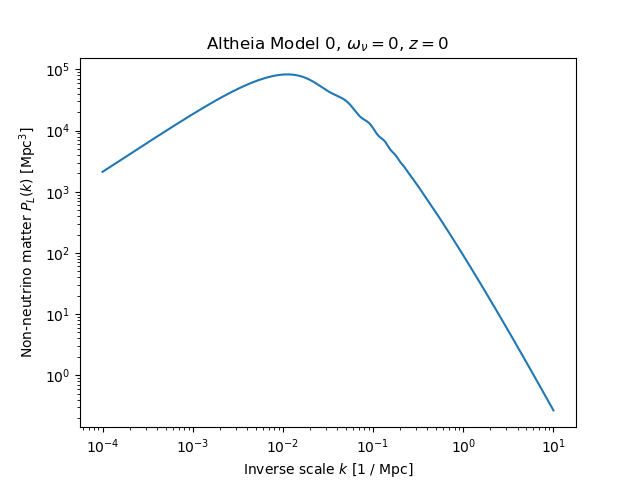
\includegraphics[scale=1.0]{intro/m0_Pk}
  \caption[Aletheia Model 0 Power Spectrum]{This is power spectrum was
  computed by CAMB for Aletheia model 0 without massive neutrinos.
  Table~\ref{tab: Aletheia_m0} defines this model in terms
  of the parameters essential to this work.}
  \label{fig: first_power_spectrum}
\end{figure}

\begin{table}[htb]
\centering
\begin{tabular}{l|l}
\hline
Parameter & Value \\ \hline
$\omega_b$ & 0.022445 \\
$\omega_c$ & 0.120567 \\
$n_s$ & 0.96 \\
$\sigma_{12}$ & 0.82476153 \\
$A_s$ & $2.1272 \cdot 10^{-9}$ \\ \hline
\end{tabular}
 \caption[Aletheia Model 0 Parameters]{This table describes
 figure~\ref{fig: first_power_spectrum} in terms of the parameters
 essential to this work. $A_s$ is truncated to five significant figures.
 Model 0 is a helpful benchmark model because it uses
 best-fit values from the Planck CMB measurements. Aletheia model 0 does not
 itself specify a physical density in neutrinos, but we will typically use
 $\omega_\nu = 0$. Unlike the rest of model 0, this setting is strongly 
 	discounted by our current cosmological observations.}
 \label{tab: Aletheia_m0}
\end{table}

A standard Planck $\Lambda$CDM model is shown in
figure~\ref{fig: first_power_spectrum}. The turnover scale $k_\text{eq}$
(eq~\ref{eq: turnover}) marks
the transition between the radiation- and matter-dominated epochs, as
$k_\text{eq}$ is the first (and therefore) smallest Fourier mode to enter the 
comoving particle horizon $\chi_h$ during the era of matter domination, where

\begin{equation}
\chi_h = \int_0^{t_0} \, \frac{dt}{a(t)}
\end{equation}

Figure~\ref{fig: first_power_spectrum} also shows the baryon acoustic
oscillation (BAO) as a set of shallow wiggles on inverse scales of roughly
$0.04 < k \, \text{Mpc} < 0.2$. The BAO is beyond the scope of this paper but,
briefly put, is the signature of a shock wave generated during the epoch of
radiation domination before baryons decoupled from photons. As baryons
collapsed into dark matter gravitational potential wells, the radiation
pressure eventually became high enough to reverse the collapse.

%s Everyone else uses h units. Why don't we?

Experienced readers will notice that our power spectrum in
figure~\ref{fig: first_power_spectrum} does not use the customary $h$ units:
our $x$-axis uses units of Mpc$^{-1}$ rather than $h$ Mpc$^{-1}$ and our
$y$-axis uses units of Mpc$^3$ rather than Mpc$^3 \, h^{-3}$. This is yet
another instance of customary factors of $h$ (see also the $\Omega_i$ and
$\sigma_8$ discussions in section~\ref{sec: param_glossary}). As mentioned
for $\sigma_8$, these units were introduced in the times when GRS redshift 
ranges justified the use of equation~\ref{eq: comov_dist_approx}. This
convention also persists in emulator literature (see, for example,
\cbib{Arico} and \cbib{Mancini}).

% The following plots were generated with h_units_bad.ipynb
\begin{figure}[htb]
    \begin{subfigure}{0.45 \textwidth}
    \centering
 		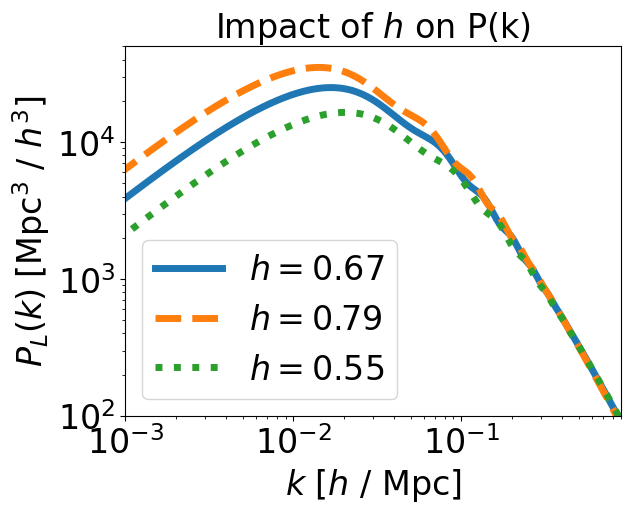
\includegraphics[width=\textwidth]{intro/h_impact_h_units}
 		\caption{Using $h$ units.}
 		\label{fig: h_units}
    \end{subfigure}
    \begin{subfigure}{0.45 \textwidth}
    \centering
 		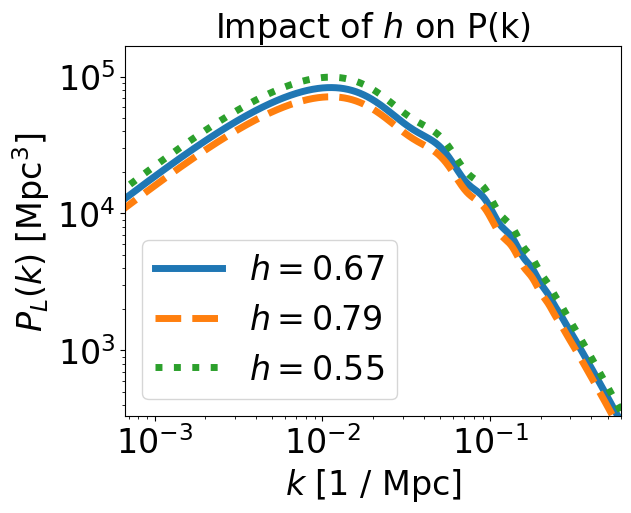
\includegraphics[width=\textwidth]{intro/h_impact_absolute_units}
 		\caption{Using absolute units.}
 		\label{fig: without_h_units}
    \end{subfigure}
        \centering
    \caption[Impact of $h$ on $P(k)$]
    		{Non-neutrino matter power spectra at $z=0$ for three different
    		models based on model zero (refer to table~\ref{tab: Aletheia_m0} 
    		for details) and varying only in the value of $h$. These two
    		panels
    		differ only in the units used. Observe that, in absolute units, we
    		can easily identify the impact of $h$ as a simple change in
    		amplitude. The use of $h$ units obscures this effect. This figure 
    		is an imitation of figure 1 from \cbib{San20}.}
    \label{fig: h_unit_Pk}
\end{figure}

%! Try to more carefully explain why it doesn't work: h is not a parameter
% over which we emulate--sigma12 is. Therefore we cannot show h in the final
% plots. This is a much subtler issue than the h complaints in the
% previous section.

Again, we refer the reader to \cbib{San20} for a detailed case against the
use of $h$ units in observational cosmology. We illustrate in
figure~\ref{fig: h_unit_Pk} one significant problem related to the
unstable meaning of $\sigma_8$: varying $h$ changes not only the power 
spectrum, but also the axes used to represent the power spectrum. Comparison 
of power spectra from different 
models is hindered because the $x$ and $y$ axes correspond to different ranges
for each curve. If we use instead units of Mpc, then changes in $h$ change
only the power spectrum, and we can much more readily appreciate its true
impact (that of an amplitude change).

As with our choice of $\sigma_{12}$ instead of $\sigma_8$, our choice of
absolute units will facilitate the application of evolution mapping described
in~\ref{sec: ev_mapping_intro}. Since $h$ only affects the amplitude of the
power spectrum, we do not need to train our emulator over it at all. Absolute 
units are not only clearer but allow us to confine all of the significance of
the value of $h$ to its impact on the value of $\sigma_{12}$.

\section{Boltzmann Solvers and CAMB}
\label{sec: boltzmann_intro}

%s What kinds of equations do we need to solve?

The power spectrum can be predicted with great accuracy via linear 
approximations. However, the evolution equations are involved (running, for
example, over many different cosmological parameters) and can be
stiff, which calls for different approaches in different regimes. Furthermore,
its solutions are highly oscillatory and therefore susceptible to numerical
errors (\cbib{Seljak}). Full solutions consist of many different steps, whose
descriptions fall outside of the scope of this work. We refer readers curious
about these equations to the history in the introduction of \cbib{Seljak},
which cites papers important to their development. 

%s Equations are hard. Who can save us?

The so-called \textit{Boltzmann codes} have been 
developed in order to leverage modern computational power and automate the
solution of these equations of evolution. Typically, Boltzmann codes offer as
outputs CMB spectra and matter power spectra. The latter is the focus of this
work.

%s What can our savior do?

As input, Boltzmann codes accept a set of values for different 
cosmological parameters, many of which were defined in section~\ref{sec: 
param_glossary}. Boltzmann codes enable us to pick from wide ranges of 
accepted values for these parameters and to consider the power 
spectrum for almost any combination of these parameters. Of course, there are 
still limitations. For example, CAMB does not currently support negative 
redshifts (which, we will later see, becomes a problem), and the minimum 
allowed value of $H_0$ is 1 km / s / Mpc, although slightly higher values have 
been observed to cause runtime errors in the presence of other extreme 
parameters.

%s Pics? Not so fast. Let's pick one.

Before we proceed to concrete demonstrations, it will be expedient to settle
on a single Boltzmann solver. As of today, the two Boltzmann codes
CAMB\footnote{\url{https://github.com/cmbant/CAMB}} and
CLASS\footnote{\url{https://lesgourg.github.io/class_public/class.html}} offer
the largest suites of features and are also actively developed. CAMB and
CLASS were written in different languages (Fortran-90 and C, respectively)
but both come with Python wrappers. These codes have been shown to be in 
excellent agreement with each other (see \cbib{Lesgourges}), and their
differences consist primarily of different approaches in algorithms (including 
speedup tricks) and user interfaces and customization options.

As the researchers in our group have much more experience with CAMB, we 
elected to use CAMB as a starting point for our Python package
Cassandra-Linear. In principal, to maximize the generality of 
the results introduced in this 
work, we would demonstrate their compatibility with at least CLASS as well. In 
practice, since these codes agree so well, we prioritize other lines of 
inquiry
for this work. However, later, in section~\ref{sec: generate_emu_data}, we 
will concede an important, 
independent reason to consider use of CLASS, which becomes a promising route
for continuation of this work (see section~\ref{sec: future_work}).

\begin{comment}
\textcolor{green}{Furthermore, the CLASS documentation
is not nearly as strong as it is with CAMB, and we already encountered
extreme difficulty simply in recreating results already previously obtained
via CAMB!}
\end{comment}

%s Examples of great results from Boltzmann solvers

\textcolor{blue}{To hint at what's to come, I start off this section by noting that several cosmological parameters have a fairly unique impact on the shape of the power spectrum, while others have a degenerate impact. Wouldn't it be great if we could know what the power spectrum would look like if we increased parameter $x$? Boltzmann solvers can help us with that.}

To connect this section with~\ref{sec: param_glossary}, we can visualize the
impact of each of this work's core parameters on the power spectrum. One
simple way to set this up for parameter $\Theta_i$ is to designate Aletheia 
model 0 as a middle ground and to create two copies of model 0, with each
copy tweaked to have an increased or decreased value of $\Theta_i$. This
approach works for every parameter except for $\omega_\nu$, where one of the
copy cosmologies describes the middle ground since the default value
$\omega_nu = 0$ is already at a hard boundary.

When feeding these cosmologies into CAMB, our Boltzmann solver of choice, we
obtain figures~\ref{fig: omega_b_dependence}, \ref{fig: omega_c_dependence}, 
\ref{fig: n_s_dependence}, \ref{fig: A_s_dependence}, and \ref{fig: 
omega_nu_dependence}. Keep in mind that the value ranges that we have applied
here are extremely broad and have nothing to do with state-of-the-art
confidence intervals on the parameters in our Unvirse. On the 
contrary, many of the values used for these plots may be completely 
discounted. The extreme values help us to clearly show the impact of each
parameter.

It should be
clear to the reader that each parameter has a special impact on the power
spectrum. None of these parameters is completely degenerate in the others,
although in the case of massless neutrinos $A_s$ and $\sigma_{12}$ are
completely degenerate, which is why we have not included an analogous plot for
$\sigma_{12}$ (the other reason being that CAMB does not accept $\sigma_{12}$
as an input--see section~\ref{sec: generate_emu_data}.

The remaining parameters $\sigma_{12}$ and $A_s$, as well as the quantities 
$z$ and $h$, all shift only the amplitude of the power spectrum. We show the 
amplitude shift associated with various $A_s$ values in figure~\ref{fig: 
A_s_dependence} and stress that the same plot only needs to be relabeled in 
order to illustrate the impact of $\sigma_{12}$, $z$, $h$, etc. 

\begin{figure}[htb]
  \centering
  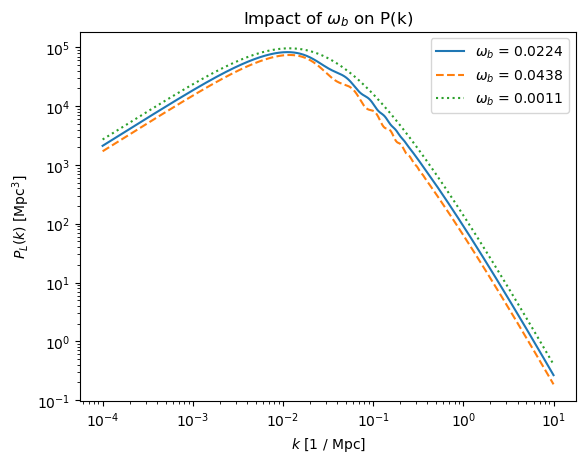
\includegraphics[scale=1.0]{intro/parameter_demos/ombh2_impact_on_Pk}
  \caption[Impact of $\omega_b$ on $P(k)$]{Impact of $\omega_b$. Increased
  	density in baryons corresponds to an increase in power on all scales.
  	However, this is not equivalent to a simple change in overall amplitude.
  	One counterexample is the shape of the BAO feature, which becomes more
  	pronounced for lower densities. A second counterexample is the location
  	of the turnover scale $k_s$, which is determined by the physical density
  	in baryons. However, this effect is subtle since the $x$-axis is
  	logarithmic and since even extreme values (relative to modern confidence
  	intervals) of $\omega_b$ will only slightly shift $k_s$. This shift
  	cannot be easily seen with the values used here.} 
  \label{fig: omega_b_dependence}
\end{figure}

\begin{figure}[htb]
  \centering
  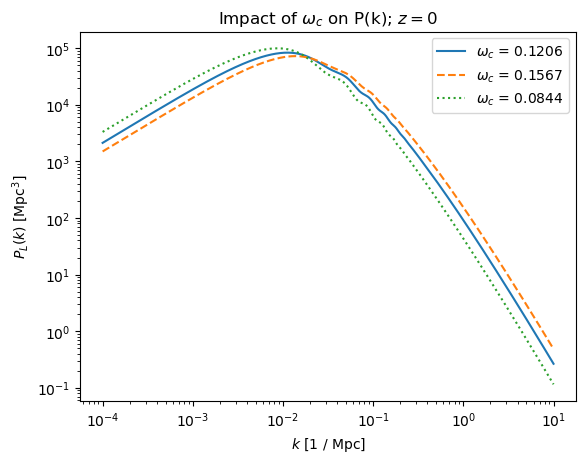
\includegraphics[scale=1.0]{intro/parameter_demos/omch2_impact_on_Pk}
  \caption[Impact of $\omega_c$ on $P(k)$]{Impact of $\omega_c$. Increased
  	density in CDM smooths out the BAO, similarly to the baryon case
  	(see figure~\ref{fig: omega_b_dependence}). More visibly, higher
  	densities shift power from larger to smaller scales due to gravitational 
  	collapse. Importantly, this behavior cannot be seen in the other
  	gravitationally interacting species, the baryons
  	(figure~\ref{fig: omega_b_dependence}). This is because, for all three
  	values used here for $\omega_c$ and for all three values used in
  	figure~\ref{fig: omega_b_dependence} for $\omega_b$,
  	$\omega_c > \omega_b$. This means that the baryon distribution will
  	largely be determined by the dynamics of CDM, rather than the
  	other way around. The dominant gravitationally-interacting species will
  	control the gravitational transfer of power from large to small scales.}
  \label{fig: omega_c_dependence}
\end{figure}

% If the gravitational collapse story were really true, why wouldn't that
% also apply to baryons? Maybe it's because b is so outnumbered by c

\begin{figure}[htb]
  \centering
  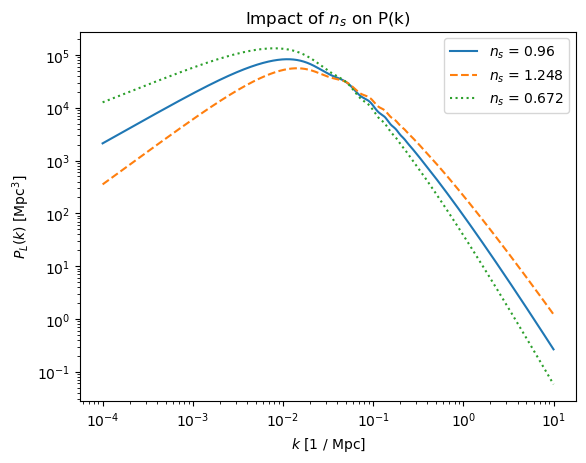
\includegraphics[scale=1.0]{intro/parameter_demos/n_s_impact_on_Pk}
  \caption[Impact of $n_s$ on $P(k)$]{Impact of $n_s$. The $n_s$ can be
  thought of as a kind of rotation of the power spectrum, although this
  is only coarse description. The differences shown here are
  adequately captured by equation~\ref{eq: n_s}.}
  \label{fig: n_s_dependence}
\end{figure}

\begin{figure}[htb]
  \centering
  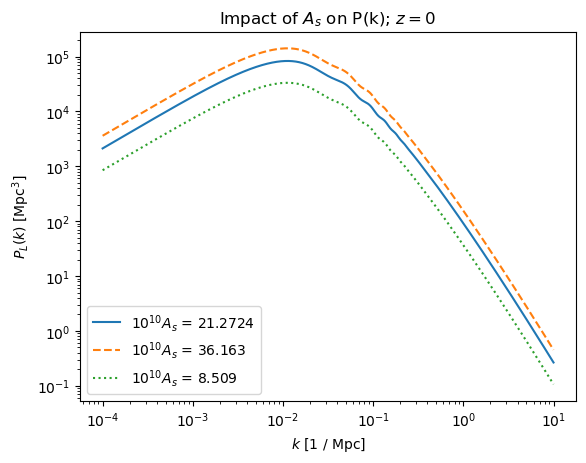
\includegraphics[scale=1.0]{intro/parameter_demos/A_s_impact_on_Pk}
  \caption[Impact of $A_s$ on $P(k)$]{Impact of $A_s$. Differences produce
  	only a change in the overall amplitude of the power spectrum. We stress
  	that this simple description applies only in the case of massless
  	neutrinos. The more subtle impact of $A_s$ will be demonstrated in
  	chapter~\ref{chap: A_s}. In the massless case, $A_s$ is completely
  	degenerate with $h$ (see figure~\ref{fig: without_h_units}) and with
  	$\sigma_{12}$ (not shown). This degeneracy is central to evolution
  	mapping, which will be discussed in section~\ref{sec: ev_mapping_intro}.}
  \label{fig: A_s_dependence}
\end{figure}

\begin{figure}[htb]
  \centering
  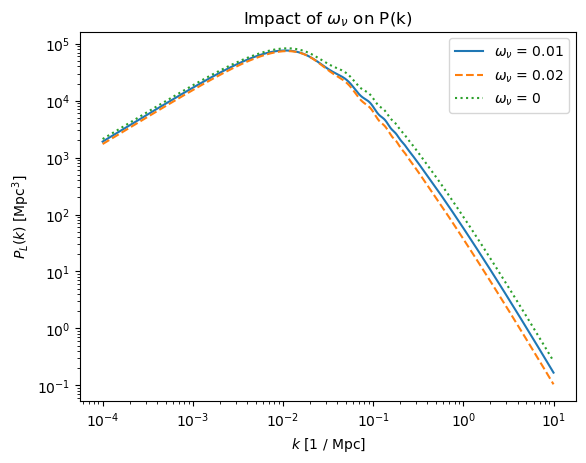
\includegraphics[scale=1.0]{intro/parameter_demos/omega_nu_impact_on_Pk}
  \caption[Impact of $\omega_\nu$ on $P(k)$]{Impact of $\omega_\nu$ for a
  	fixed redshift. $\omega_\nu$ is not like other parameters--combining
  	a change in $\omega_\nu$ with a change in $z$ is not a simple sum of the
  	operations. This sounds awkward, let's rewrite...}
  \label{fig: omega_nu_dependence}
\end{figure}

%s Segue into the next section

Since many of these parameters have fairly unique impacts on the power 
spectrum, we can imagine building a collection of power spectra labeled by
their parameter configurations and then comparing our real-world observations 
to them. We can ask to which of these theoretical power spectra our 
observations most closely agree. This question is quantitatively answered by 
parameter inference in the form of a Monte Carlo Markov Chain (MCMC) analysis, whose basic idea will be discussed in the next section.


\section{Monte Carlo Markov Chains}

This can be a very brief section, but I want to discuss a little bit of how most modern parameter inference works because it motivates the need for extremely fast power spectrum computation. It provides a sort of conceptual bridge between our ``pure'' goal (quantifying the cosmos) and the nitty-gritty bulk of the paper (optimizing emulator performance).

Metropolis-Hastings algorithm.

We don't know what the true probability distribution of power spectra is. In order to build this distribution with simulation results, we simply draw from the distribution. \textcolor{orange}{Refer to ``Data to Insights'' lecture notes in order to tighten this description.}

\section{Emulation: Basic Principles}
\label{sec: emulation_intro}

To conduct these MCMC analyses, we need several thousands of power spectra. However, if our Boltzmann solvers take on the order of three seconds to run, then these solvers will become the bottleneck of our analysis. \textcolor{orange}{Give some specific numbers for this.}

This motivates the introduction of emulation, basically multi-dimensional interpolation, in order to predict the power spectra. These predictions are orders of magnitude less time-expensive. 

Emulators interpolate across a high-dimensional parameter space. The primary
limitation is that the emulator has to be built with every possible parameter
in mind that an end-user could wish to vary. Yet there is a large number of
different cosmological parameters discussed in the modern literature.
``Currently available emulators only sample a few cosmological parameters,
often with restrictive ranges, and are not applicable to more general
parameter
spaces'' (\cbib{San21}). ``Due to the high computational cost of the required
simulations, [...] current emulators leave out parameters such as the
curvature
of the Universe or dynamic energy models beyond the standard CPL
parametrization'' (\cbib{San21}).

I'll talk a little about different emulators currently available, such as COMET. Some emulate non-linear power spectra, for example, and several even include massive neutrinos. But this thesis will demonstrate that massive neutrinos can be included into our evolution mapping approach, which will be introduced in section~\ref{sec: ev_mapping_intro}.

% (This is good news because the evolution mapping approach greatly simplifies the parameter space, and enhances the accuracy), which is the subject of the next section.

\section{Gaussian Process Regression}
\label{sec: gpr_intro}

% What is a Gaussian Process?

Most emulators are based on a Gaussian Process (GP). A GP is a Gaussian
distribution over functions\footnote
{A GP is the limit of a one-hidden-layer neural network as the number of
neurons approaches infinity.}, which can be interpreted
as the infinite-dimensional generalization of the multivariate normal
distribution. The inference of continuous values with a GP prior
is known as Gaussian process regression, or Kriging. GP regression is a
powerful non-linear multivariate interpolation tool. The computational
complexity of inference and likelihood evaluation within GP regression is cubic
in the number of points. This makes GP regression an excellent companion to
Latin hypercube sampling (LHS), which makes highly efficient use of a limited 
number of samples and whose basic idea will be explained in section~\ref{sec:
lhc_theory}.

Neural networks (NNs) generally need much larger sample sizes to reach
comparable levels of
accuracy. Due to various alterations in the Cassandra-Linear code over its
development, several regenerations of the various emulator data sets were
necessary. This practical constraint motivated the use of a GP for our
emulator. Furthermore, NNs invariably require much more complicated setup and
tuning--for example, in the precise architecture of the network (e.g. nodes
per layer, layer types) as well as the hyperparameters (e.g. learning rate).
By contrast, as we explain in section~\ref{sec: train_emu}, a Gaussian
process regression is highly straightforward to set up and modify. Therefore,
for a demonstration project such as Cassandra-Linear, we elected to base our
emulator on a GP. Please refer to the section~\ref{sec: future_work} for a
continuation of this discussion.

Are there other prediction approaches besides GPs and NNs? IF so, I need to
further justify WHY we’re using GPs.
GPs work best when there are few samples and a lot of parameters, right?
But why is that so? What is the math behind that?


\section{Sampling Approach: Latin Hypercube}
\label{sec: lhc_theory}

I imagine this is going to be an extremely short section. We should motivate why we're using this style of sampling.

What is the theoretical best LHC that we could make?

Besides, can we explain this equation?


\section{Evolution Mapping}
\label{sec: ev_mapping_intro}

\textcolor{blue}{I want to briefly summarize why we can funnel all of the 
evolution parameters through $\sigma_{12}$ in this way. This objective may be
too ambitious for this paper, because I would have to go through each
evolution parameter and derive its evolution nature in a few lines of 
equations.} \textcolor{orange}{Maybe I can just do the same thing as Ariel
recommended with the GPR kernel: ``we played around and found that this
works.''}

(\cbib{San21}) proposes to divide up the full set of cosmological
parameters into two categories: \textit{evolution} parameters $\mathcal{O}_E$
(such as $\omega_b$, $\omega_c$, and $\eta_s$)
affect the amplitude of the power spectrum at a particular redshift, while
\textit{shape} parameters $\mathcal{O}_S$
(such as $\omega_K$, $\omega_\text{DE}$, w(a))
affect the shape of the power
spectrum.

We take, as the evolution mapping relation for the power spectrum, equation 13
from \cbib{San21}:

\begin{equation}
\label{eq: evMapping_pSpectrum}
    \Delta^2_L (k | z, \Theta_s, \Theta_e)
    =
    \Delta_L^2 (k | \Theta_s, \sigma_{12} \left( z, \Theta_s, \Theta_e \right))
\end{equation}\footnote{Varying $z$ has the same effect as varying an
evolution parameter, which is why it appears on the RHS only as an argument to
the $\sigma_{12}$ ``function.'' We write it separately from $\Theta_e$ to
emphasize that $z$ does not describe a property of the Universe, but is
simply used as a proxy here for \textcolor{red}{conformal?} time
\textcolor{red}{elapsed since the Big Bang? (but we can only observe up to
$z = 1100$...)}.}

Why is this scheme important? Evolution mapping greatly simplifies the emulator
implementation. Because we can
funnel all of the evolution parameters through $\sigma_{12}$, we've effectively
collapsed an entire category of parameters to just one parameter. Fewer
parameters means that we get a more accurate emulator.

``At the linear level, all models characterized by identical shape parameters
and the same values of the parameter combinations $b \sigma_{12}(z)$ and
$f \sigma_{12}(z)$ will be identical'' (\cbib{San21}).

Now, for the hiccup, which segues into the next section: this scheme is broken by one parameter, the Universe's
density in neutrinos. (In the next section: why this is so and what we can do
about it.)


\section{Neutrinos and Their Cosmological Impact}

\begin{figure}[htb]
  \centering
  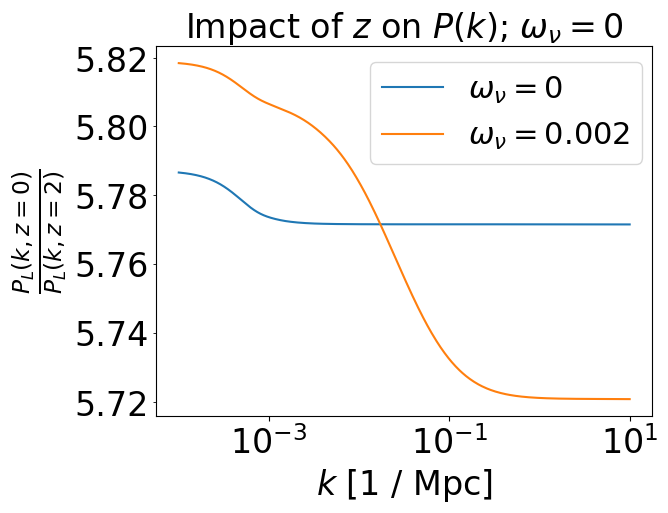
\includegraphics[scale=0.5]{intro/redshift_dependence_problem}
  \caption[Redshift Dependence of Neutrino Impact]{Blue is also not flat,
  	quite surprisingly.}
  \label{fig: neutrinos_and_redshift}
\end{figure}

(\cbib{Kiakotou}): ``Neutrinos with masses on the eV scale or below will be a
hot component of the dark matter and will free-stream out of overdensities and
thus wipe out small-scale structures.''

``In general, a larger density of relativistic species leads to a smaller
growth of matter fluctuations'' (\cbib{Zennaro}).

The point of this section is: why is $\omega_\nu$ bad for the
evolution mapping scheme? Because neutrinos exhibit redshift-dependent
damping of the power-spectrum, and therefore affect both the shape and the
amplitude of the power spectrum. Whenever massive neutrinos are present,
the growth factor becomes scale-dependent, which disrupts the
evolution-mapping scheme.

Why do they behave in this way? All neutrinos start off as
relativistic particles in the early Universe, acting as a type of radiation.
But as the Universe continues to expand and cool, the neutrinos behave
increasingly like dark matter.
In this way, the physical density in neutrinos impacts both the shape and the
evolution.

``The popular heuristic formula for the linear theory suppression of the matter
fluctuations by free-streaming $\nu$, $\Delta P(k) / P(k) \approx -8 f_\nu$, is
valid only on very small scales $k > 0.8 h$ / Mpc, However, it is not of
practical use as this is in the strongly nonlinear regime of matter
clustering'' (\cbib{Kiakotou}).

One proposed solution is to treat the neutrinos as a small correction factor
to the results from an anologous cosmology with the same $\omega_m$ but with
$\omega_\nu = 0$. This of course limits the applicability of our emulator to
cosmologies with very small $\omega_\nu$, but this constraint agrees with
current observations (\textcolor{orange}{which?}).

I want to end this section with a vague plan of action: we want to play around with CAMB power spectra to see if there are any simple ways around this limitation in our approach.

%%% New stuff

% what is a MEMNeC?

We already have an approximation for the power spectrum of a massive-neutrino cosmology within the evolution mapping scheme. The $\sigma_{12}$ value that we described earlier is actually the $\sigma_{12}$ value of the model's MEMNeC. can already be approximated within evolution-mapping by slightly altering scheme. \textcolor{red}{Is it fair to say we are adjusting, or was this actually the same scheme as it always was?} We take a MEMNeC and the desired cosmology. The sigma 12 is actually the sigma 12 of the MEMNeC. Then we treat the physical density in neutrinos as a shape parameter along with $A_s$.

  \chapter{CAMB, Initial Setup}

%%%%%%%%%%%%%%%%%%%%%%%%%%%%%%%%%%
%%  Beispiel fuer eine Tabelle  %%
%%%%%%%%%%%%%%%%%%%%%%%%%%%%%%%%%%

\begin{table}[htb]
\centering
\begin{tabular}{l|l}
Erste Spalte & Zweite Spalte \\ \hline
Eintrag & Eintrag
\end{tabular}
 \caption[Kurzform f"ur das Tabellenverzeichnis]{Dies ist die Erkl"arung zur Tabelle.}
\end{table}

CAMB is a Fortran code with a Python wrapper\footnote{
\url{https://github.com/cmbant/CAMB}
}which we will be using for the
entirety of this project.

To introduce the reader to the scope of CAMB, we will now introduce
some basic simulated power spectra along with a summary of the dynamic
parameters which will be of greatest interest to us.

I hope to, in painstaking detail, cover many of the lines of the code that I
have written to interface with CAMB. I will include plots to indicate, at
every step, what incorrect settings cause the power spectrum to look like (or,
for subtler errors, what the error curves looked like compared to Ariel's
results, which I treated as a sort of ``ground truth''). This should also be a
good example to flex my physics interpretation skills: why does this incorrect
setting produce this undesired pattern?

You might think that this is sort of an inappropriate section for a master's thesis (especially since I have in mind that this be a lengthy section), but I would like to include it unless you feel very strongly. After all, I spent several months of the project debugging at least ten different ways that slight and major errors in the various settings led to irreconcilable results.

For example, one parameter that tripped me up for a while: neutrino mass hierarchy: the options are degenerate, normal, and inverted. The CAMB documentation annotates this parameter as ``(1 or 2 eigenstate approximation),'' but this is somewhat unclear. Is the degenerate hierarchy the single mass eigenstate approximation? Do both normal and inverted hierarchies involve two eigenstates?

%In figure \ref{fig: spectrum_type}, we can see that requesting of the wrong
%power spectrum type can in some low-$\omega_\nu$ cases yields errors so low
%that we might accidentally overlook them. This error pattern is easily
%recognizable and is a consequence of the definition of the power spectrum: the
%Fourier transform  of the two-point correlation function. ...Okay, I'm still thinking about this. I don't understand %yet, but I'll be sure to ask you if I'm still struggling about it.

Another paragraph I want to have in this section: stress the part of the evolution mapping introduction, that the $\sigma_{12}$ value we're using to describe the model is actually the $\sigma_{12}$ value of the model's MEMNeC! This is so important and confusing that maybe I'll even recapitulate again later in the section on the generate\_emu\_data.script.

%%% New stuff

Beware the neutrino settings. The effective number of massive neutrinos is about 3.027

%! This is weird, and perhaps inappropriate for a thesis document.

To test this setup, we compare our results with those of Ariel S\'{a}nchez and
Andrea Pezzotta for the first seven Aletheia cosmologies and four physical
densities in neutrinos, for a total of 28 models. The errors are miniscule and
recorded in figure XXY. After verifying the accuracy of our code in this way,
we proceed to experiment with the power spectra in order to explore solutions
to the evolution mapping problem.
  \chapter{Expansion of the Parameter Space}
\label{chap: A_s}

Now that we have a comprehensive set of convenience functions with which to
configure CAMB, we can easily obtain the theoretical power spectra we need in
order to demonstrate our solution to the neutrino difficulties introduced in
section~\ref{sec: neutrino_problem}. This chapter will motivate the inclusion 
of the additional parameter $A_s$ in the evolution mapping framework.
Because the focus of this thesis is regression rather than theory,
we will merely show that $A_s$ contains information relevant to the impact of
massive neutrinos. Then, the GPR should, in principle, be able to optimize its
use to predict power spectra.

% Maybe it would make more sense to have the large cass-L chapter focus on the
% creation of a massless-neutrino emulator and THEN a smaller chapter focusing
% on all the changes necessary for it to become a massive-neutrino emulator.
% BUT! As of 25-08-23, I'm running way behind on writing actual content for
% this thesis. I can't risk redoing all the section headers again. We're
% going to proceed under the current scheme and MAYBE allow ourselves to redo
% it shortly before submission.

\section{Equation to be Solved}

% Redo section title

\textcolor{orange}{Remember to explain \textit{why} the prediction of these 
asymptotes means that $A_s$ will capture most of the unruly behavior of 
neutrinos. What theory motivates such a judgment? Or are we only guessing?}

We begin with the second proposal from section~\ref{sec: neutrino_problem}:
to approximate the power spectrum of a massive-neutrino cosmology, we use the
power spectrum of its MEMNeC. This can be represented symbolically as

\begin{equation}
\label{eq: MEMNeC_approx}
P_\nu(k) \approx P_0 (k)
,\end{equation}

Where $P_\nu (k)$ is the power spectrum of the massive-neutrino cosmology in
which we are interested and $P_0(k)$ is the power spectrum of its MEMNeC.

Consider that the exact relation is trivially

\begin{equation}
P_\nu(k) = \de(k) \, P_0 (k)
,\end{equation}

where $\de(k) \equiv P_\nu (k) / P_0 (k)$.

The essence of this chapter is to increase the accuracy in our $P_\nu(k)$
predictions by estimating $\de(k)$.

To visualize the problem, we have plotted $P_\nu (k) / P_0(k)$
in figure~\ref{fig: ratio_plots} for model 0 at two redshifts.

Since approximation~\ref{eq: MEMNeC_approx} worked reasonably
well, we know that

If we can estimate $\el$ accurately, then in principle our task 
is complete, because the slope toward smaller $k$ values is
even and analytically predictable. \textcolor{green}{Can I refer the reader to
 a paper on this?}

The differences are a little large, so we study a subtler
quantity $\ee_i (k)$:

\begin{equation}
\ee_i (k) \equiv \frac{\de_\text{model i}(k)}{\de_\text{model 0}(k)}
\end{equation}

To simplify our demonstrations, we will concentrate on the
small-scale limit of this ratio $\el_i$

\begin{equation}
\el_i \equiv \lim_{k \rightarrow \infty} \ee_i(k)
\end{equation}


\section{Proposed Fitting Functions}

\textcolor{orange}{This section, like the ``Convenience Functions'' section
from chapter 2, should anticipate CL: we should talk about the
code that we have written in order to explore these ratios, which one can find
in} \verb|camb_interface.py|.


The \verb|model_ratios| function.

The \verb|model_ratios| function goes in the section where we conclude that 
$A_s$ and $\omega_\nu$ suffice to capture the growth factor suppression of 
massive neutrinos.


\section{Testing Functions}

The \verb|get_As_matched_cosmology| function.
The \verb|get_random_cosmology| function.

In producing asymptote plots, we find that our predictions line up quite well,
but not perfectly. This may indicate that our parametrization is insufficient.
In other words, we may need additional cosmological parameters besides the
$A_s$ and $\omega_\nu$ and in order to fully characterize the impact of
massive neutrinos on the power spectrum.

However, the imperfect performance of our predictions may also simply
indicate that the final form of our asymptote predictions (equation XXY) is
only an approximation of some true (or at least more accurate) relationship
between $A_s$, $\omega_\nu$, and the small-scale suppression of the power
spectrum. A symbolic regression investigation could prove highly effective at
resolving this ambiguity by efficiently searching out improved formulas. 
However, we do not consider this a promising avenue
for the continuation of this work (see section~\ref{sec: future_work} for our
recommendations), because the error on our predictions is so low. The error
is so low here that we do not believe the imperfect predictions to
significantly detract from the performance of the emulator.

\section{Summary of Findings}

% I'm not sure if this section will survive, we'll see how big the conclusion
% here ends up being.

So, our massive-neutrino emulator will be trained over six cosmological
parameters: $\omega_b$, $\omega_c$, $n_s$, $\sigma_{12}$, $A_s$, and
$\omega_\nu$. In other words, to predict a power
spectrum $\hat{\vec{y}}$, the emulator will accept as an input $\vec{x}$
these six parameters.

%s Now segue into the next chapter

We just need to add $A_s$ to the set of cosmological parameters
over which we train our GPR and then we can treat $\omega_\nu$ like a shape
parameter. Expansion of the parameter space represents the single most 
important novel step in this work. The remaining chapters will
focus on the integration of this new approach into a beginner-friendly
emulation code.

  \chapter{Conceptual Outline of Our Emulator Code and Pipeline}

\textcolor{blue}{The point of this section is to introduce the reader to the
basic structure of the emulator pipeline. Most of the discussion will follow
from a flow chart showing the various conceptual pieces of the emulator. Also
in this section, I will introduce various choices made (e.g. 5000 training
spectra, 300 points for each spectrum) WITHOUT justifying any of them--later,
in chapter~\ref{chap: disc_and_conc}, we'll justify these decisions and
talk about the consequences of alternate settings.}

In order to simplify the process of testing different emulator setups, and to make power
spectra more accessible to beginners in the field, we have developed a Python package,
which we call Cassandra-Linear (CL)1. CL represents a full emulation pipeline from the
generation of training and testing data to the plotting of error statistics associated with
the emulation.

% We're gonna need a flow chart for this puppy. That should be priority number
% one, because the writing should constantly refer back to it.

\section{Design Choices}

By default, each Latin hypercube consists of $N_s = 5000$ entries. For 
justification of this quantity, please refer to
section~\ref{sec: num_samples}.

$N_k = 300$.

\section{Creation of Separate Emulators}
\label{sec: 2emu_intro}

\textcolor{blue}{This is a brief introductory section motivating the creation 
of two emulators:
unlike the other five parameters, the physical density in massive neutrinos 
has a hard lower bound. This creates some minor regression problems (appeal to 
boundary effects / danger of extrapolation).}

One potential weakness of \textcolor{orange}{this} emulator outline emerges 
from the prior range for the physical density in neutrinos. The lower bound 
($\omega_\nu = 0$) of this range for the physical density in neutrinos is 
highly firm; any negative value would be totally unphysical. However, this 
lower bound is also inclusive in the sense that the massless neutrino case is 
still very much of interest to us. GP predictions are, naturally, at their 
strongest in the regions densest with training samples. Since the massless 
neutrino case represents the end of a parameter range, the sampling must be 
less dense there. Indeed, no massless-neutrino cases are even in our training 
sample, XXX being the minimum value of $\omega_\nu$ in our 
LHS.\footnote{\textcolor{orange}{What should I say to people who complain: 
``why not just manually add massless-neutrino samples to the original training 
set? Why not simply have one emulator trained over a more diverse training 
set?'' I think it would be better if we simply focus on the $\omega_\nu = 0$
case not being adequately captured by interpolation, since we don't have any
samples on the ``left'' side of $\omega_\nu = 0$.}}
Therefore, the massless-neutrino case is actually \textcolor{green}{a slight
extrapolation} from our training data, which is dangerous for accuracy.

To 
address this unique problem among our parameter ranges, CL can automatically 
access one of two emulators depending on the user’s input. The primary 
emulator is trained over the aforementioned prior range in $\omega_\nu$
(table~\ref{tab: neutrino_priors}). In addition to this, we’ve trained a 
separate emulator specifically to handle the massless neutrino case. In 
practice, this entails the same prior ranges for the parameters $\omega_b$, 
$\omega_c$, $n_s$, and $\sigma_{12}$. However, here we no longer need $A_s$;
as discussed in chapter~\ref{chap: A_s}, $A_s$ helps to characterize the
structure growth suppression induced by massive neutrinos. Besides this, for 
the purposes of our training and validation data, $A_s$ is redundant since it
is otherwise an evolution parameter, and we are already specifying the 
amplitude of the power spectrum through sigma12. 

To train this massless-neutrino emulator, we use the same code as described in 
in this chapter and chapter~\ref{chap: implementation}. Since the
massless-neutrino emulator is trained over just four parameters, and since we 
nevertheless continue to train over 5000 samples, we expect the
massless-neutrino emulator to be universally more accurate. However, as
discussed and plotted in section~\ref{sec: num_samples}, our decision to train 
over 5000 is justified by the rapidly diminishing returns in additional 
accuracy.

\textcolor{orange}{The following paragraph is bad. I'm not sure yet if I can
salvage anything. The claims are not true and the work is not yet done.}

Therefore, the reason why the massless-neutrino emulator is more 
accurate is because massive neutrinos in particular have a highly complicated 
impact on the power spectrum. Even with the inclusion of the $\omega_\nu$ and 
$A_s$ parameters, our investigations in chapter~\ref{chap: A_s} reveal that
these two parameters may not be sufficient to fully characterize the 
suppression of the power spectrum by massive neutrinos. Of course, we would 
like to reiterate that, though we have applied a symbolic regression approach 
in order to independently justify our analytical expression from
chapter~\ref{chap: A_s}, this by no means guarantees that we have found the optimal analytical expression.

To simplify the user experience, this two-emulator solution lives ``under the
hood'' and by default \textcolor{orange}{will be} hidden behind an interface
which automatically queries the correct emulator given some user-input
cosmology.

To justify our decision and to quantify the improvement from this approach, we
have prepared \textcolor{orange}{some} plots in section~\ref{sec: 2emu_improvement}.

\textcolor{orange}{Conclude this section by saying that this integration of multiple emulators into one user-facing script can be further exploited with, for example, different emulators for different neutrino mass hierarchies.}

Besides its relevance to the neutrino suppression of the small-scale power
spectrum, $A_s$ appears to be an evolution parameter. Therefore, when the
emulator discussion branches into the massless- and massive-neutrino cases
(refer to section~\ref{sec: 2emu_intro} for the beginning and motivation of
this), the reader should keep in mind that the dimension of the parameter
space decreases in the massless-neutrino case by \textit{two}--$\omega_\nu$ 
obviously must vanish because we here assume $\omega_\nu=0$. However, $A_s$
also vanishes because, without massive neutrinos, $A_s$ reduces to an
evolution parameter and is therefore redundant with $\sigma_{12}$.

% What happens to A_s in the massless-neutrino case? Is it fixed at the
% default for model 0? I'm pretty sure it is!


\section{Unit LHCs}
\label{sec: lhc_flow_chart}

The \verb|pyDOE2| function that we will use to generate our LHCs
returns a result with entries that range from zero to unity. We will refer
to such LHCs as \textit{unit} LHCs.\footnote{We will later denote LHCs with 
the matrix notation $\matr{X}$ and collections of CAMB power spectra as
$\matr{Y}$ to
emphasize the roles of these data in the training and testing of the emulator. 
However, we will continue to use the term ``unit'' as introduced here, and 
the reader should keep in mind that a unit $\matr{X}$ therefore does not
indicate an identity matrix.} These unit LHCs will eventually be used 
to create a set of cosmological configurations which will act as the $X$ data 
set when we train our emulator.

In order to these LHC entries into cosmological parameters that we can input 
into CAMB, we will need to rescale them with our priors for each parameter.
However, instead of rescaling immediately, we will rescale later: 
\textcolor{orange}{The benefits of rescaling later are. This is useful not
just for changing priors but even for changing the way that we sample a
particular prior (for example, $\sigma_{12}^2$ sampling--although we did not
get it to work, the infrastructure is still there for whoever comes along in
the future.}
 
We describe the building of the unit LHC in section~\ref{sec: build_lhc}
and its rescaling (as well as the construction of the $Y$ data set) 
in~\ref{sec: generate_emu_data}.


\section{Default Priors}
\label{sec: default_priors}

% One reason this goes here: priors show up in almost every script,
% so there isn't a great cass-L section in which to put this.

As we will explain in section~\ref{sec: build_lhc}, our code generates unit 
Latin hypercube samples so that a single hypercube can be used to build 
several different emulators simply by using a different set of priors to 
rescale the cube.

CL is packaged with three pairs of prior files. Depending on which priors the 
user selects, the emulator will automatically become a massive-neutrino or 
massless-neutrino emulator. \textcolor{orange}{This needs to be linked to the 
convenience section, on how to add scenario files and what not. But this 
feature is not finished yet! We may have to punt it to “future work.”}

\textcolor{orange}{Table goes here.}
% Caption for one table: The ``classic'' priors represent a middle ground 
% between those of ``COMET'' and ``MEGA''.

In tables XXX-XXZ, we provide the specific upper and lower bounds for each of
the six cosmological parameters over which our massive-neutrino emulator is 
trained. All intervals are sampled uniformly, \textcolor{orange}{Although some
experimental code exists to interpret the same hypercube as a uniform sampling
in root or square space, for example}. At first, we used the highly ambitious 
(relative to modern uncertainty bars) ``MEGA'' set of priors
(table~\ref{tab: priors}),
whose values we decided based on the recent emulator papers from
\textcolor{green}{Spurio Mancini et al 2021. and the other paper, I can't
remember the name.} However, during the process of generating training data, 
we found that CAMB was not able to match all of the necessary $\sigma_{12}$ 
values. We refer to such a situation as an unsolvable cell, and will explain
why it happens in section~\ref{sec: generate_emu_data}, which covers the
application of evolution mapping principles within the CL code.

\textcolor{orange}{Talk a little more about the prior ranges, what are their
values in words??}

The default priors that we use correspond to those currently used by COMET. \textcolor{orange}{Two
justifications for this choice: unsolvable cells, but more than that, simplicity and accuracy
for the ``demo'' run.}

\section{Emulation over Uncertainties}

\textcolor{orange}{I'm nominating this section for deletion. I doubt I'll have
the time to put together a fully-fledged uncertainty emulator...}

For a further step of accuracy, we can add a third data set to our pipeline
and introduce a second layer of emulation.

Up to this point, our pipeline has included a training set and a testing set.
If we add a validation set, then we can train a second emulator over the
errors associated with the first emulator's performance on this validation
set.

Within the current (as of \textcolor{orange}{24.08.2023}) setup of
Cassandra-Linear, we typically generate two Latin hypercubes for each
emulator. The first represents our training set and an emulator cannot be
produced without it. The second one represents our validation set.

\textcolor{orange}{In a future
release of Cassandra-Linear, this set will be used to train an ``uncertainty''
emulator, which will train over the errors from the main emulator in order to
provide the user with an uncertainty estimate for any cosmology located within
the space of priors over which the main emulator was trained.} 

\textcolor{orange}{However, this functionality has not yet been implemented. 
Currently, we are 
using the validation hypercube more as a test hypercube: we compute the uncertainties at discrete points and examine these uncertainties (e.g. with
scatterplots and histograms) to assess the performance of the emulator.}

  \chapter{Results and Analysis}
\label{chap: results}

In this chapter, we will discuss the performance of a two-emulator setup
built using the default configuration of CL: both the massless- and
massive-neutrino emulators appraised here use the COMET priors
(table~\ref{tab: COMET_priors}), $N_k = 300$, and $N_s = 3000$ for both the
training and testing data sets.

\section{Quantifying the Performance of the Emulator}

To evaluate the performance of the emulator, we use the testing pipeline
explained in section~\ref{sec: test_emu}.
That is, we create an LHS of test cosmologies, which the training stages have
never seen, and compare the output of the emulator object to that of
CAMB. As in neural network contexts, GPR performance is typically evaluated
using test sets (\citealp{Mancini}, \citealp{Arico}, and
\citealp{Eggemeier}).\footnote{However, these test sets are
more commonly referred to as ``validation sets.'' We use the phrase
``test set'' to call to mind the three conventional data sets in a machine
learning setup: training, validation, and testing. This distinction will
prove useful in section~\ref{sec: future_work}.}

We appreciate that appraisal based on test sets
may not provide hard boundaries on the true
range of errors associated with the emulators,
because the continuity of the parameter hypervolume means that an infinite
number of cosmologies could be tested. Therefore, traditional
goodness-of-fit tests such as $\chi^2$ do not apply here.
However, precisely because
power spectra vary smoothly in this space\footnote{Indeed, without this
property, interpolation would be unproductive.}, we expect the error 
curves to vary similarly. So long as the test LHS represents a reasonable
coverage of the parameter space, we expect the errors calculated therefrom to
be similarly representative of emulator performance. On the other
hand, at the edges of the parameter space, where interpolation begins to
break down, the errors will be at their highest, and the following analyses
may not be representative of these edge cases.

For this chapter as well as chapter~\ref{chap: disc_and_conc}, we will focus
on just two error metrics: percent error and squared error. We include percent
error as it is more common in the literature and because it is immediately
interpretable (\citealp{Mancini}, \citealp{Arico}, and
\citealp{Eggemeier}). By contrast, the squared errors are difficult to
understand unless compared across multiple similar cases.
Nevertheless, we argue
that squared errors represent a more useful metric, at least within a single
paper, because they are unbiased with respect to the magnitude of the emulated
quantity. Consider that $P(k)$ is smallest at the largest $k$; if an emulator
mispredicts $P(k)$ with a constant offset, then the percent error curves will
be largest at the smallest $k$. As a further example, consider that the
overall amplitude of $P(k)$ is smaller for smaller $\tilde{\sigma}_{12}$;
if we again imagine a constant offset, $\tilde{\sigma}_{12}$ will appear as a
problematic parameter if we look only at percent error.


\section{Percent and Absolute Errors on Random Cosmologies}

\begin{figure}[ht!]
  \centering
  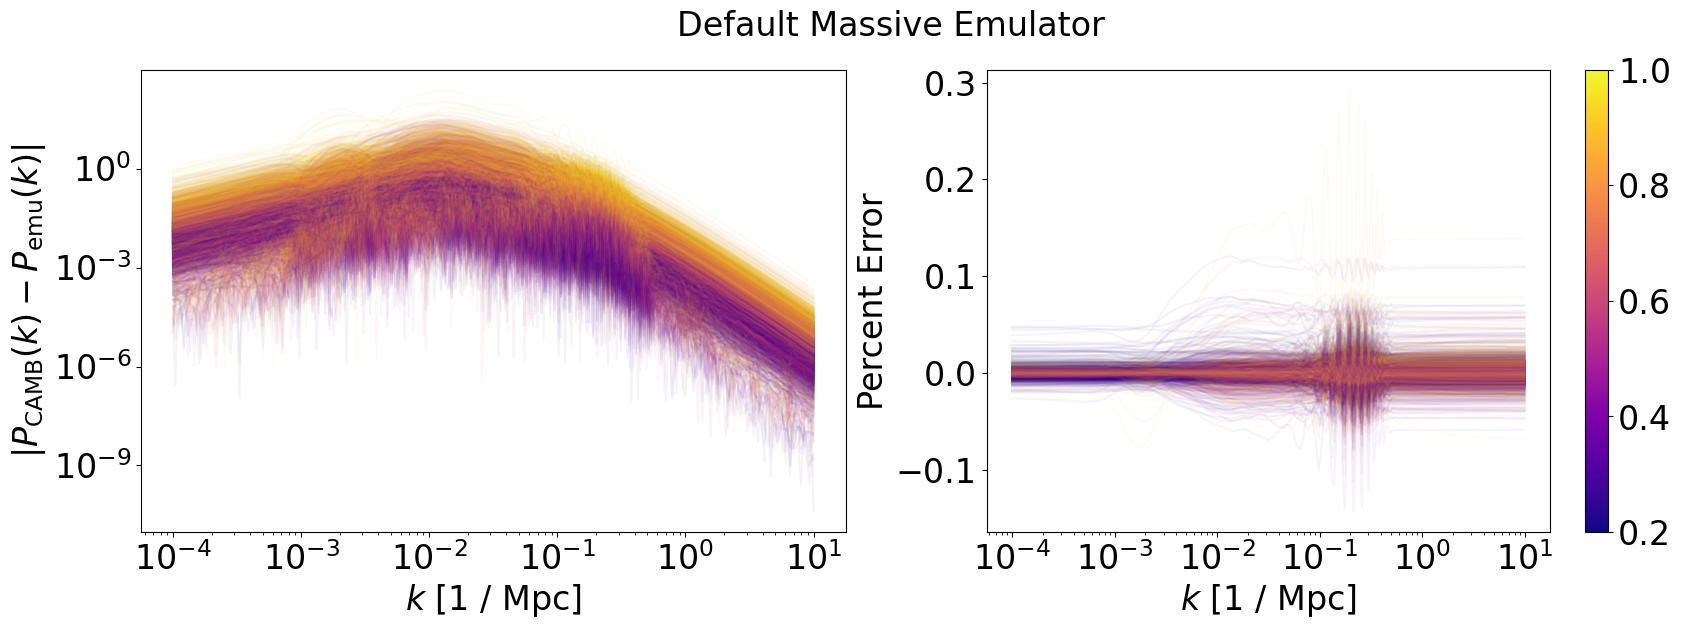
\includegraphics[width=\textwidth]{error_on_emulators/def_massive_curves}
  \caption[Default Massive Emulator Error Curves]{5000 error curves provided 
  by running the test set through the emulator. The curves are colored
  according to their value in $\tilde{\sigma}_{12}$. The opacity of the curves
  allows us to conclude that the dynamic range, at least in the percent
  error case, is dominated by a small number of cosmologies.
  In absolute terms, the emulator
  clearly performs best on the small scales. In relative terms, the
  performance is best on large scales. Regardless of the metric used, the
  error is most extreme on medium scales, and drastic fluctuations can be seen 
  in the percent error plot.}
  \label{fig: def_massive_curves}
\end{figure}

\begin{figure}[ht!]
  \centering
  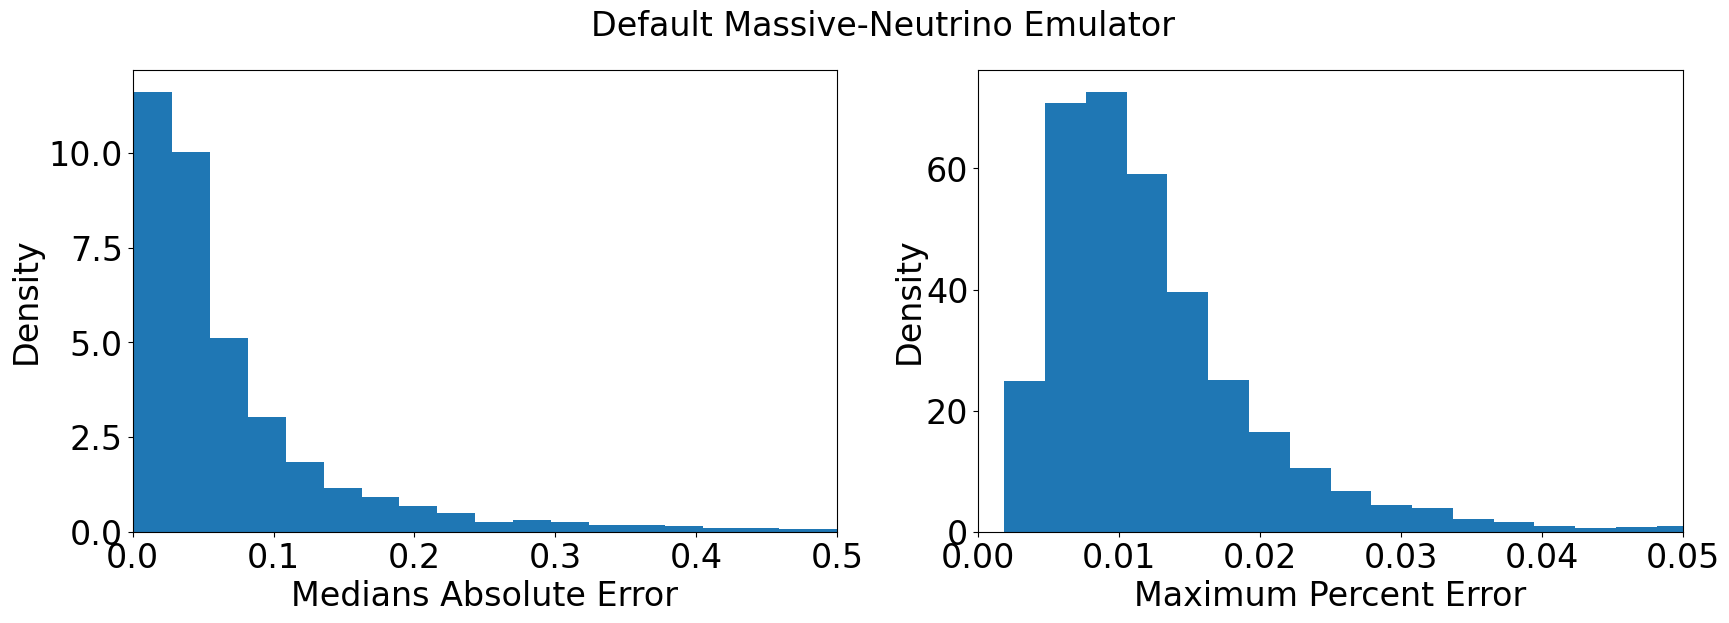
\includegraphics[width=\textwidth]{error_on_emulators/def_massive_hist}
  \caption[Default Massive Emulator Error Histograms]{The left plot is a
  	histogram of the medians of the absolute values of each difference curve.
  	The right plot is a histogram of the maxima of the absolute values of
  	each percent error curve. In both cases, we find the plots to have
  	extremely long tails, so we have truncated these plots at arbitrary
  	right endpoints in order to focus on the central shape.}
  \label{fig: def_massive_hist}
\end{figure}

In figure~\ref{fig: def_massive_curves}, we 
show the performance of the default massive-neutrino emulator. We consider
the overall performance encouraging. Even the worst error curve, which
appears to have been the worst by far, did not exceed a 0.3\% error.
In the follow-up histograms (figure~\ref{fig: def_massive_hist}), we find
that in the vast majority of tested cosmologies, the error does not
exceed 0.04\%.

The curves of figure~\ref{fig: def_massive_curves} were colored according to
their values in $\tilde{\sigma_{12}}$, which we found was the only parameter
associated with a consistent trend. At large scales, lower values of
$\tilde{\sigma}_{12}$ are associated with higher percent errors. However, at
all scales, higher values of $\tilde{\sigma}_{12}$ are strongly tied to
increased absolute error.

The dramatic
oscillations around the BAO region suggest to us that improving the emulator's
handling of the BAO would be the most promising avenue for tightening the
overall distribution of error.

\begin{figure}[ht!]
  \centering
  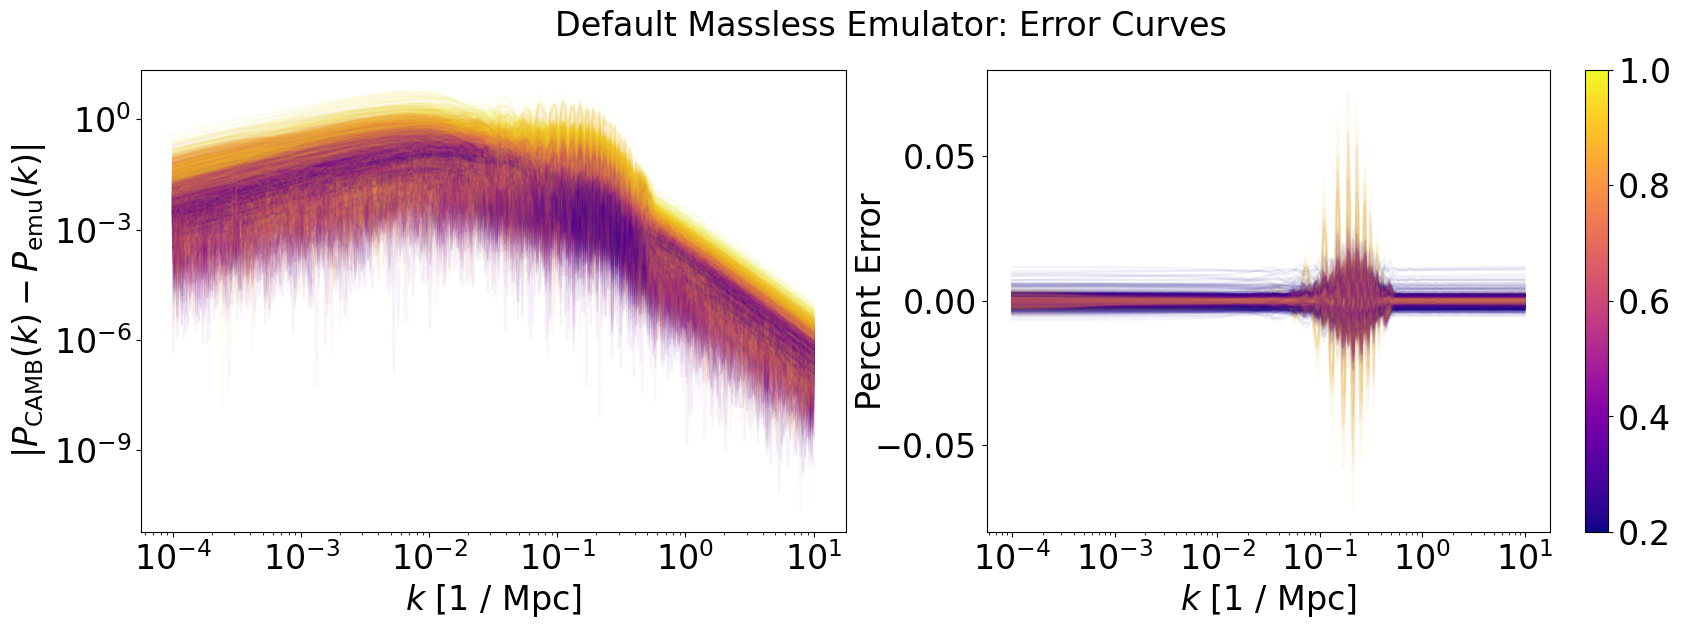
\includegraphics[width=\textwidth]{error_on_emulators/def_massless_curves}
  \caption[Default Massless Emulator Error Curves]{5000 error curves provided 
  by running the test set through the emulator. The curves are colored
  according to their value in $\tilde{\sigma}_{12}$.
  In absolute terms, the emulator
  clearly performs best on the small scales. In relative terms, the
  performance is about the same on large and small scales.
  Regardless of the metric used, the
  error is most extreme on medium scales, and drastic fluctuations can be seen 
  in the percent error plot.}
  \label{fig: def_massless_curves}
\end{figure}

\begin{figure}[ht!]
  \centering
  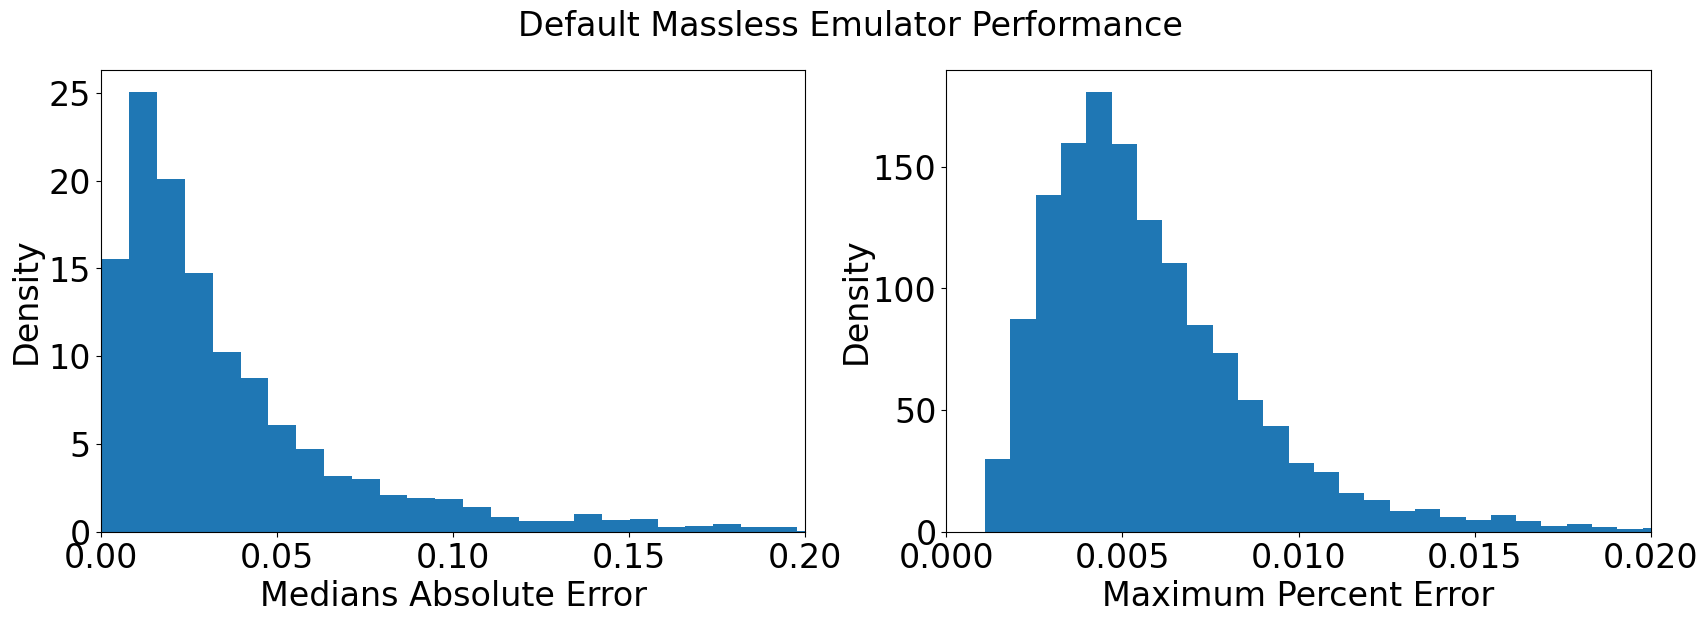
\includegraphics[width=\textwidth]{error_on_emulators/def_massless_hist}
  \caption[Default Massless Emulator Error Histograms]{1000 error curves provided by running the test set through the emulator.}
  \label{fig: def_massless_hist}
\end{figure}

In figures~\ref{fig: def_massless_curves} and~\ref{fig: def_massless_hist},
we have included analogous plots from our massless-neutrino emulator.
The overall shape of the error curves appears similar to the massive
case, although here the absolute errors are small enough that fluctuations
in the BAO region can be clearly seen in both cases. Furthermore, the
percent error curves appear to be tightly concentrated both at small and
large $k$, whereas the spread towards large $k$ increased visibly
in the massive case. From the histograms we can appreciate that the error
distributions are roughly similar but the spread has been tightened in both
histograms by roughly a factor of two. By contrast, the percent error
curves have decreased in dynamic range by a factor of four.

The BAO fluctuations are proportionally much more significant here, suggesting
that the BAO errors are the most significant contributor to percent errors
across all cosmologies. This
further encourages future work to focus on BAO modeling, as both the massive-
and massless-neutrino emulators could benefit significantly.

\textcolor{orange}{Create some plots focusing on the BAO error spikes? i.e.
zoom-in on k-ranges.}

The massive emulator clearly performs worse than its 
massless counterpart. The emulators are difficult to compare because they
were constructed from LHSs of different dimension: four in the massless case,
six in the massive case. Since $N_s = 5000$ is constant, we expect the 
massless LHS to sample the parameter space much more densely than the massive
LHS. In any case, the discrepancy in accuracies will be worsened by the
approximate nature of our fit from section~\ref{sec: proposed_fit}:
the results of section~\ref{sec: fit_testing} indicate
that evolution parameters besides $A_s$ are necessary for complete
characterization of the impact of massive neutrinos. Nevertheless, the
overall percent error of the massive emulator is comparable with that
of CAMB itself, so we consider the massive emulator a confirmation of the
techniques introduced in chapter~\ref{A_s}.

\textcolor{orange}{I plan to spend some time talking 
about \textit{why} parameter x is the current biggest problem for the 
emulator.}

\textcolor{orange}{It would have been nice if you had done like Andrea said,
and produced a plot colored by the ``extremeness'' of the parameters. We
could implement an extremeness index for parameter $x$ simply by taking
subtracting 0.5 and taking the absolute value, assuming that $x$ comes from
the unit LHS. Then, we could take the average over six parameters to get
an extremeness index for the cosmology as a whole. Optionally, for plot
optimization, you could multiply the final value by 2 so that the extremeness
runs from 0 to 1.}


\section{Improvement from Two-emulator Solution}
\label{sec: 2emu_improvement}

\begin{figure}[ht!]
  \centering
  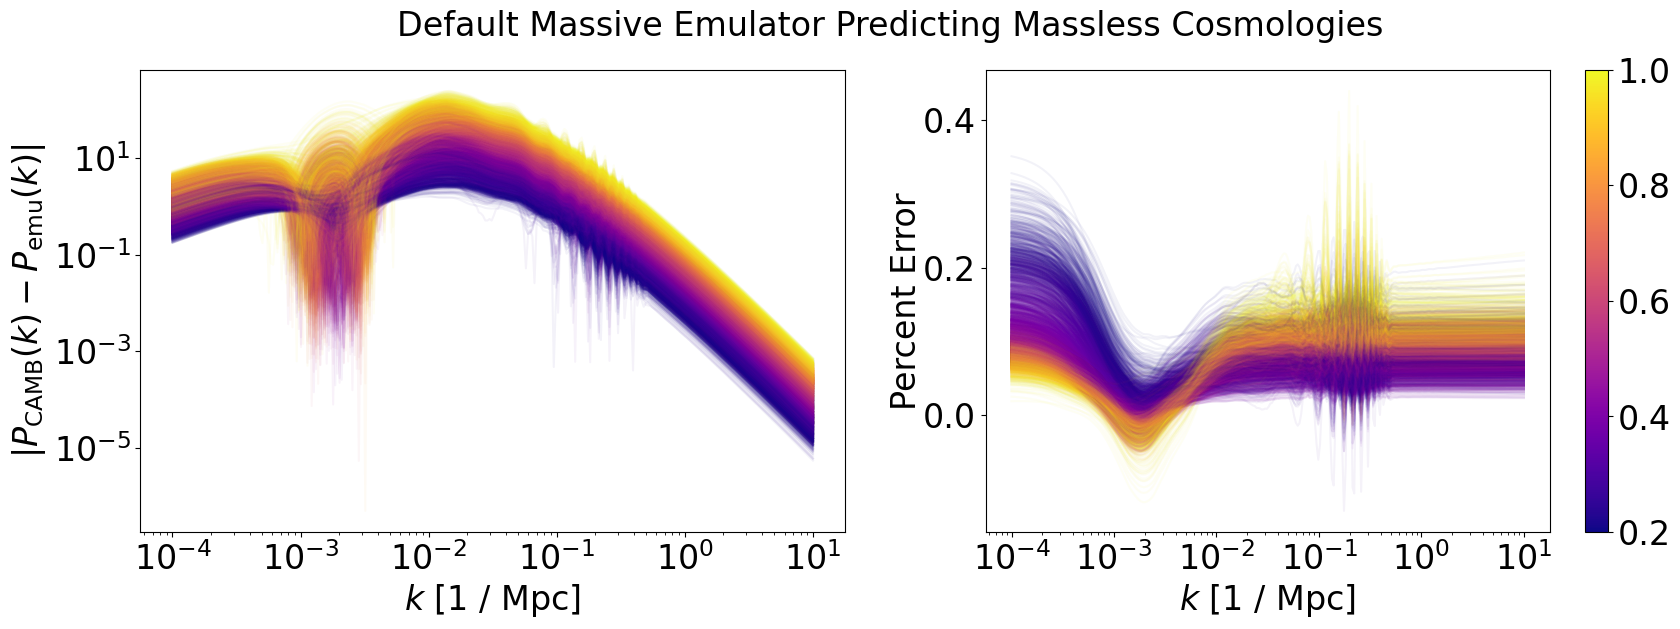
\includegraphics[width=\textwidth]{error_on_emulators/two_emu_curves}
  \caption[Performance of Massive Emulator in Massless Case]{1000 error
  	curves provided
  	by running the massless-neutrino test set through the massive-neutrino 
  	emulator. The shape of both plots is significantly different from the
  	massive-emulator's test cosmologies shown in
  	figure~\ref{fig: def_massive_curves}. We therefore consider our
  	two-emulator solution strongly motivated.}
  \label{fig: two_emu_curves}
\end{figure}

To justify our use of a two-emulator solution to increase
accuracy in the massless-neutrino case, we task the massive-neutrino emulator 
with predictions over the test set of the massless-neutrino emulator.
To adjust the four-dimensional massless-neutrino test LHS to
the six-dimensional massive-neutrino emulator, we filled in
$A_s \approx 2.1272 \cdot 10^{-9}$ and $\omega_\nu = 0$ everywhere.
We consider
this a fair test because we sampled $\omega_\nu$ values for the
massive-neutrino emulator from a uniform distribution [0, 0.01]. Therefore,
in principle, the $\omega_\nu = 0$ case should only be a slight extrapolation.

The overall error of the massive emulator is larger, but this does not
explain all of the results that we see--these error curves also differ
significantly in shape, with increasingly aberrant behavior at large scales.
Also, the BAO feature seems to be slightly complicated by the presence of
massive neutrinos.

Now that we have used the massless-emulator test set to motivate our use of
a two-emulator solution, we move on from the massless emulator.
As evolution-mapping emulation for \textit{massive}-neutrino cosmologies
is the novel feature of this work, we will henceforth concentrate exclusively
on the massive-neutrino emulator.

\section{Minimum Separation of the Training LHC}
\label{sec: error_from_lhc}

The final training LHS had an $s^*$ of 0.07972 in the massive case and 
0.02274 in the massless case. The final testing LHS had an $s^*$ of 0.07275 in 
the massive case and 0.02015 in the massless case. All numbers have been 
rounded to four significant figures.

What is the impact of the minimum separation? Surely the minimum separation
should be a proxy for the evenness of the coverage of the space of
cosmologies. Therefore, we expect the error variance to increase much more
dramatically than, say, the average bias.

How would we be able to quantify the error due to this? We could try to 
compare the emulator performance trained on hyper cubes of various minimum 
distances.

% The following plots were generated with emu_experiment_histograms.ipynb
\begin{figure}[ht!]
    \begin{subfigure}{0.35 \textheight}
    \centering
 		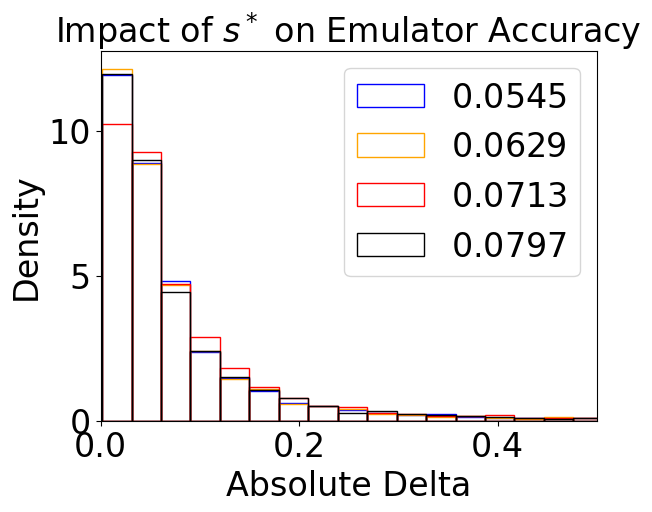
\includegraphics[width=\textwidth]{error_on_emulators/deltas-hist-minsep}
 		\caption{Median absolute errors.}
 		\label{fig: minsep_experiment_deltas}
    \end{subfigure}
    \begin{subfigure}{0.35 \textheight}
    \centering
 		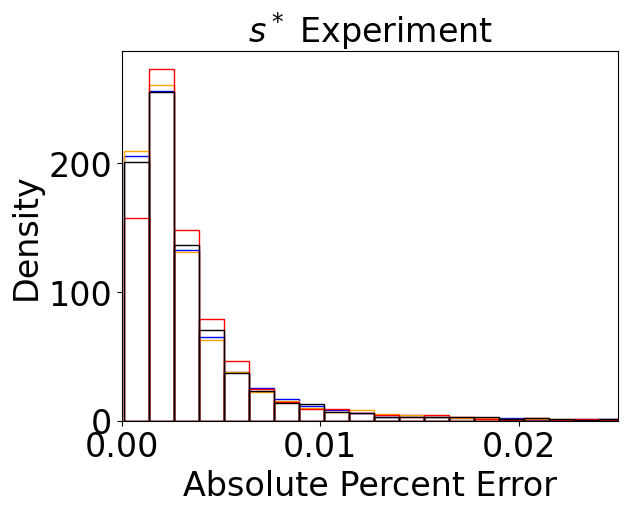
\includegraphics[width=\textwidth]{error_on_emulators/percents-hist-minsep}
 		\caption{Median absolute percent errors.}
 		\label{fig: minsep_experiment_percerr}
    \end{subfigure}
        \centering
    \caption[Impact of $s^*$ on Accuracy]
    		{Histograms of errors associated with emulators trained on LHSs of
    			different $s^*$ values. Doesn't seem to make much difference. For the tested values, see
    			table~\ref{tab:}.}
    \label{fig: minsep_experiment}
\end{figure}

% The following table was generated with emu_experiment_stats.ipynb
\begin{table}[ht!]
\centering
\begin{tabular}{l|l|l|l|l}
\hline
$s^*$ & Median of Means & Median of Medians & Median of STDs & Maximum PTP \\ \hline
$0.0545$ & 0.167753 & 0.045098 & 0.232575 & 205.656917 \\
$0.0629$ & 0.169627 & 0.044320 & 0.234392 & 174.772714 \\
$0.0713$ & 0.194701 & 0.050606 & 0.275545 & 203.590333 \\
$0.0797$ & 0.173023 & 0.044955 & 0.244320 & 224.434379 \\
\end{tabular}
	\cprotect\caption[$s^*$ Experiment: Percent Error Statistics]{Lower is
		better. The
		results of this experiment are surprising. We consider that there
		may have been an error in our execution of the experiment...
		None of the statistics shows a trend consistent with our expectations,
		and only in the case of the median of medians is the last-row value
		lower than that of the first row.}
 \label{tab: minsep_experiment_delta_stats}
\end{table}

% The following table was generated with emu_experiment_stats.ipynb
\begin{table}[ht!]
\centering
\begin{tabular}{l|l|l|l|l}
\hline
$s^*$ & Median of Means & Median of Medians & Median of STDs & Maximum PTP \\ \hline
$0.0545$ & 0.002835 & 0.002240 & 0.002025 & 0.192945 \\
$0.0629$ & 0.002850 & 0.002179 & 0.002079 & 0.196711 \\
$0.0713$ & 0.003052 & 0.002409 & 0.002059 & 0.266151 \\
$0.0797$ & 0.002883 & 0.002255 & 0.002058 & 0.291348 \\
\end{tabular}
	\cprotect\caption[$s^*$ Experiment: Percent Error Statistics]{The
		results of this experiment are surprising. We consider that there
		may have been an error in our execution of the experiment...
		we find it a strange coincidence that the percent errors steadily
		get worse... perhaps the effect is so subtle that we would have to
		run more experiments?}
 \label{tab: minsep_experiment_percerr_stats}
\end{table}

\section{Resolution of the k Axis}

This might go better in the CassL section, but I think I ought to motivate the 
decision to use length-300 arrays.

\begin{figure}[ht!]
  \centering
  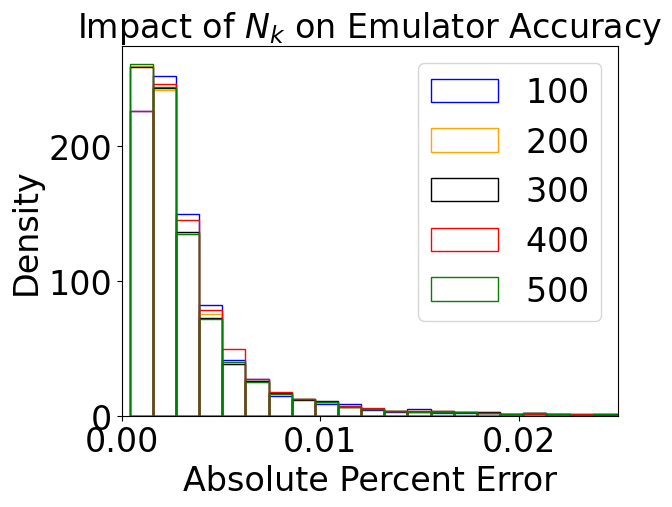
\includegraphics[scale=0.5]{error_on_emulators/percents-hist-N_k}
  \caption[Impact of $N_k$ on Accuracy]{The test is too fair!}
  \label{fig: Nk_experiment}
\end{figure}

This is a special case where we would argue that percent error is more useful 
than squared error.
That is because percent error can be considered on its own, whereas squared
error relies on comparison for its meaning to emerge. But in this case, the
comparisons are obscure. Consider, for example, comparing an $N_k = 100$
emulator with an $N_k = 500$ emulator: the $N_k = 100$ emulator will have
fewer points from which to compute errors. Simple interpolation is not enough
to restore direct comparability, as the $N_k = 500$ emulator by definition
will suffer less from interpolation than the $N_k = 100$ emulator, for which
each point will have to inform five times as much as the interpolated function
domain.

% The following table was generated with emu_experiment_stats.ipynb
\begin{table}[ht!]
\centering
\begin{tabular}{l|l|l|l|l}
\hline
$N_k$ & Median of Means & Median of Medians & Median of STDs & Maximum PTP \\ \hline
$100$ & 0.003082 & 0.002427 & 0.002174 & 0.272042 \\
$200$ & 0.002878 & 0.002243 & 0.002054 & 0.297159 \\
$300$ & 0.002883 & 0.002255 & 0.002058 & 0.291348 \\
$400$ & 0.003034 & 0.002461 & 0.002042 & 0.277015 \\
$500$ & 0.002881 & 0.002221 & 0.002088 & 0.296367 \\
\end{tabular}
	\cprotect\caption[$N_k$ Experiment: Percent Error Statistics]{Caption!}
 \label{tab: Nk_experiment_percerr_stats}
\end{table}

\section{Number of Training Samples}
\label{sec: num_samples}

\textcolor{blue}{Justify choice of 5000 samples for each: maybe we can make a
trend plot showing diminishing returns in test error?}

% The following plots were generated with emu_experiment_histograms.ipynb
\begin{figure}[ht!]
    \begin{subfigure}{0.35 \textheight}
    \centering
 		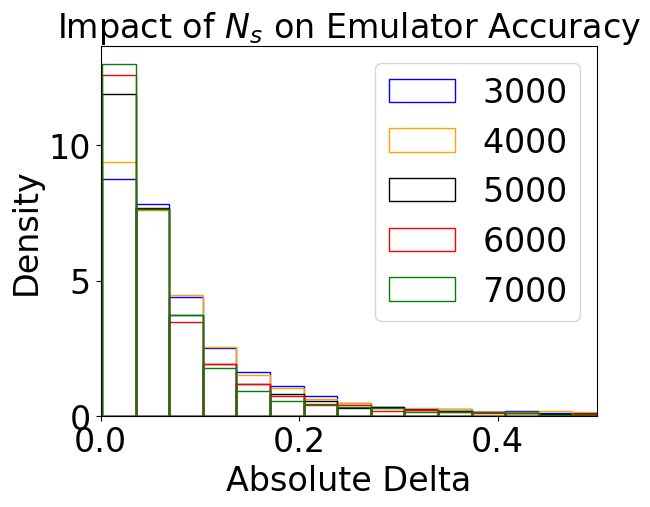
\includegraphics[width=\textwidth]{error_on_emulators/deltas-hist-N_s}
 		\caption{Median absolute errors.}
 		\label{fig: Ns_experiment_deltas}
    \end{subfigure}
    \begin{subfigure}{0.35 \textheight}
    \centering
 		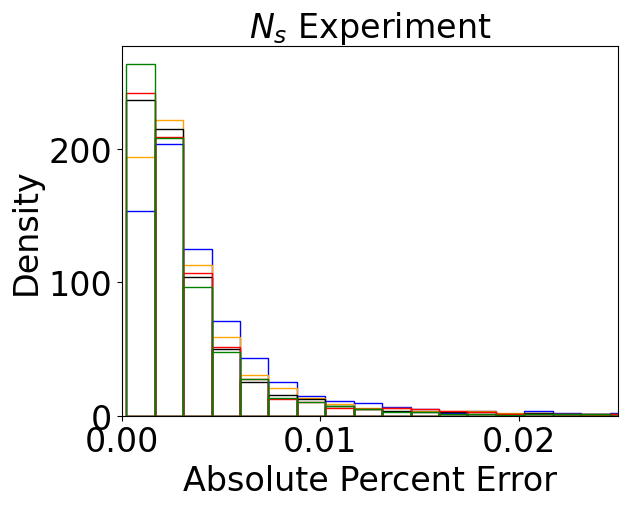
\includegraphics[width=\textwidth]{error_on_emulators/percents-hist-N_s}
 		\caption{Median absolute percent errors.}
 		\label{fig: Ns_experiment_percerr}
    \end{subfigure}
        \centering
    \caption[Impact of $s^*$ on Accuracy]
    		{Histograms of errors associated with emulators trained on LHSs of
    			different $N_s$ values. Doesn't seem to make much difference,
    			but unlike the other cases, we can definitely say here that it
    			makes a difference.}
    \label{fig: Ns_experiment}
\end{figure}

% The following table was generated with emu_experiment_stats.ipynb
\begin{table}[ht!]
\centering
\begin{tabular}{l|l|l|l|l}
\hline
$N_s$ & Median of Means & Median of Medians & Median of STDs & Maximum PTP \\ \hline
$3000$ & 0.2382 & 0.0588 & 0.3388 & 175.5588 \\
$4000$ & 0.2010 & 0.0567 & 0.2741 & 185.5470 \\
$5000$ & 0.1730 & 0.0450 & 0.2443 & 224.4344 \\
$6000$ & 0.1712 & 0.0425 & 0.2415 & 146.6090 \\
$7000$ & 0.1633 & 0.0410 & 0.2305 & 118.7862 \\
\end{tabular}
	\cprotect\caption[$N_s$ Experiment: Deltas Statistics]{This table shows
		the volatility of the last column, as the median colmuns agree on the
		trend.}
 \label{tab: Ns_experiment_deltas_stats}
\end{table}

% The following table was generated with emu_experiment_stats.ipynb
\begin{table}[ht!]
\centering
\begin{tabular}{l|l|l|l|l}
\hline
$N_s$ & Median of Means & Median of Medians & Median of STDs & Maximum PTP \\ \hline
$3000$ & 0.0037 & 0.0030 & 0.0027 & 0.2794 \\
$4000$ & 0.0032 & 0.0026 & 0.0022 & 0.2305 \\
$5000$ & 0.0029 & 0.0023 & 0.0021 & 0.2913 \\
$6000$ & 0.0028 & 0.0022 & 0.0020 & 0.1893 \\
$7000$ & 0.0027 & 0.0021 & 0.0019 & 0.1189 \\
\end{tabular}
	\cprotect\caption[$N_s$ Experiment: Percent Error Statistics]{YES!
		We caution that the last column can be a misleading statistic
		(especially because the deltas table does not show the same trend), but
		it is still a helpful value to quote...}
 \label{tab: Ns_experiment_percerr_stats}
\end{table}


% This might go better in the CassL section, but I think I ought to motivate 
% the decision to use 5000 training arrays.

\textcolor{orange}{I'll have to concede that the results of this section are 
not entirely comprehensive; we didn't train any emulators over the 
uncertainties of analogous validation hypercubes. All comparisons here use the
simpler pipeline of just two data sets, training and testing.}

  \chapter{Conclusion}
\label{chap: conclusion}

Massive neutrinos represent a challenge for evolution-mapping emulators
because their damping of the power spectrum depends on redshift.
This redshift dependence results in $\omega_\nu$ impacting both the
amplitude and the shape of the linear-theory cold-matter power spectrum.
This behavior precludes exclusive categorization as either a shape or
evolution parameter.

We find that two simple adjustments to evolution mapping can extend its
efficacy to the case of massive neutrinos. By recasting the evolution mapping
relation in terms of $\tilde{\sigma}_12$ rather than $\sigma_{12}$--that is,
in terms of the MEMNeC amplitude rather than the desired cosmology's
amplitude--we are able to circumvent the impact of $\omega_\nu$ on the
amplitude of the power spectrum, particularly on large scales. Furthermore,
we find that $A_s$ is not exclusively an evolution parameter but contains
information about the impact of massive neutrinos on the small-scale
power spectrum. By including it as a parameter over which we train the
emulator, we find that the small-scale accuracy significantly improves.

We introduce a new code, the Python package Cassandra-Linear, to construct
and test an emulator of the linear-theory cold-matter power spectrum based on
these extensions to the evolution mapping recipe. We offer a detailed survey
of the capabilities of this code so that interested readers can build and
experiment with their own emulators.

We compare the accuracies of two emulators trained using this code: one
including $A_s$ and $\omega_\nu$, and the other featuring no massive 
neutrinos. We find that the massless-neutrino emulator performs significantly
better when the number of samples is held fixed. Nevertheless, we show that
the $3\sigma$ confidence interval is below the 0.1\% error level. This means
the error of our massive-neutrino emulator is
comparable to that of CAMB, the Boltzmann solver we use to produce the
training spectra used for training.

We explore the impact of $s^*$, $N_k$, and $N_s$ on the performance of the
emulator and find...

In conclusion...

% Just use one big block of text, don't split into sections

\textcolor{red}{How do these results compare with results from 
papers on similar subjects?}

\section{Emulation over Uncertainties}

\textcolor{blue}{This content should be subsumed into future work, since we
didn't manage to complete this feature in time.}

For a further step of accuracy, we can add a third data set to our pipeline
and introduce a second layer of emulation.

Up to this point, our pipeline has included a training set and a testing set.
If we add a validation set, then we can train a second emulator over the
errors associated with the first emulator's performance on this validation
set.

Within the current (as of \textcolor{orange}{24.08.2023}) setup of
Cassandra-Linear, we typically generate two Latin hypercubes for each
emulator. The first represents our training set and an emulator cannot be
produced without it. The second one represents our validation set.

\textcolor{orange}{In a future
release of Cassandra-Linear, this set will be used to train an ``uncertainty''
emulator, which will train over the errors from the main emulator in order to
provide the user with an uncertainty estimate for any cosmology located within
the space of priors over which the main emulator was trained.} 

\textcolor{orange}{However, this functionality has not yet been implemented. 
Currently, we are 
using the validation hypercube more as a test hypercube: we compute the 
uncertainties at discrete points and examine these uncertainties (e.g. with
scatterplots and histograms) to assess the performance of the emulator.}


\section{Future Work}
\label{sec: future_work}

To conclude this work, we here identify several promising paths to advancing
both the Cassandra-Linear code as well as the scientific analyses in
chapter~\ref{chap: results}. The potential improvements are
numerous, but we here concentrate on the most important
suggestions.\footnote{For smaller suggestions, refer to the GitHub issues 
page: \url{https://github.com/3276908917/Master/issues}}.

%s Section 1: science improvements

Based on the results of sections~\ref{sec: error_from_lhc} and~\ref{sec: 
num_samples}, it would behoove future inquiries to investigate whether we
can in some way compensate for the different impact of $N_s$ on the massive
and massless emulators so that their accuracies may be directly compared.
Such a comparison would help us to understand the error associated
specifically with the evolution mapping extensions introduced in
chapter~\ref{chap: A_s}. Even if a direct comparison method cannot be
established, it would be useful to know how much larger $N_s$ would have to
be for a massive emulator to reach equivalent levels of error.

Based on the results of section~\ref{sec: error_from_lhc},
\textcolor{blue}{we do not consider LHC improvement to be a significant
priority}. But if it were... we would look through the theory. Can we build
a generator of perfect, or at least much  better, LHCs?

%s Section 2: code improvements. Segue offered by the uncertainty emulator.

We want to build an emulator over the validation set in order to quote an 
uncertainty to the user and to try to further correct for errors? I'm not sure 
I understood that last part, we would have to ask Ariel again.

\textcolor{orange}{The integration of 
multiple emulators into one user-facing script can be further exploited with, 
for example, different emulators for different neutrino mass hierarchies.}
Extend the two-emulator solution to create emulators with different mass
hierarchies. Mass hierarchy should also be an option to specify in the
scenario file, like: degenerate, normal, inverted, both normal and inverted. 
Remember to scale the mnu correctly to bridge the gap between degenerate and
normal that we observed when playing around.

(For example, $\sigma_{12}^2$ sampling--although we did not
get it to work, the infrastructure is still there for whomever comes along in
the future. This suggestion builds on the concepts of
section~\ref{sec: lhc_outline}.)

%s Section 3: use of different technologies

%s CLASS versus CAMB again

Although our priors should already suffice for most conventional parameter
inference studies, we believe that wider priors would be of benefit to those
seeking to understand exotic cosmologies. The chief obstacle to 
implementation of wider priors in CL is CAMB's requirement that $z \geq 0$. 
Negative redshifts do not violate any conditions in the equations of
cosmological evolution, so it could prove fruitful to investigate why CAMB 
has this requirement; if the code could be easily amended, the results of
this work could be extended to broader priors. Alternatively,
CLASS \textcolor{green}{allows} negative redshifts, so it may be worthwhile 
to repeat the work of this thesis using power spectra from CLASS.

Should we use a neural network instead of a Gaussian process for our emulator? 
AndreaP and Alex Eggemeier are already on the job: they are converting COMET 
to a neural network approach. We recommend that the reader follow future COMET 
papers for investigations into this question.

GP's allow natural propagation of
uncertainty in predictions to the final posterior distribution; neural
networks lack this feature. At the same time, NNs provide larger speedups 
\textcolor{green}{CITATIONS}. We performed limited testing of a neural network
but did not allocate enough time to arrive at conclusive / quantitative
comparisons.


% Inquiries using different technologies

%s Code improvements

%%% Unprofessional to mention the following here:
\begin{comment}
The code should be expanded with documentation and unit tests. Also, the
user interface script is still in progress.

To simplify the user experience, this two-emulator solution lives ``under the
hood'' and by default \textcolor{orange}{will be} hidden behind an interface
which automatically queries the correct emulator given some user-input
cosmology.
\end{comment}


\section{Tightness of the Priors Used}
\label{sec: prior_woes}

With this section I would like to revisit the specific values for the priors,
that I only briefly mentioned back in section~\ref{sec: build_lhc}.

First of all, from a purely practical consideration, expanding the priors was
not feasible due to the high incidence of unsolvable cells.

But second, this may not be a significant limitation to the utility of the
emulators introduced here, because they are already quite wide compared to
current state-of-the-art parameter inferences. \textcolor{green}{CITATIONS}.

As of 19.06.23, ``COMET'' is the default for the emulator. It is the most 
restrictive of the three options and was implemented in order to totally 
eliminate the problem of unsolvable cells, allowing us to train our 
demonstration emulator over an LHS without any significant gaps.

Our hope was that the narrow parameter ranges would furthermore help the 
demonstration emulator to achieve high accuracy--in principal, success here
means that we can simply ``scale up'' the approach of this work by
simultaneously expanding the priors as well as the total number of training
samples. Unfortunately, it is not clear if we can scale up the emulator past
the point at which unsolvable cells begin to appear. Since Latin hypercube
sampling is designed to evenly sample a space, unsolvable cells certainly
indicate that parts of the parameter space lack representation in the training
data. In these regions, our emulator will be forced to interpolate across
large gaps, or worse, extrapolate (if the unsolvable cells occur at the edges
of the parameter space \textcolor{orange}{This is something that I should have
shown... i.e. with plots}).
% Andrea recommends a plot coloring points by the "extremeness" in our sample
% space.

We predict that increasing the total number of cells will only marginally
reduce the issue of unsolvable cells \textcolor{orange}{This is something that 
I should have shown... i.e. with plots}). We can imagine the subspace of
solvable points as some hypervolume within a hypercube determined by our
priors, and the emulator's training coverage as an approximation of this 
hypervolume with small hypercubes whose size is determined by the separation 
between points in the sample. In the ideal case, the space of solvable points 
is the same as the Latin hypercube. When this is not so, we can at least
reduce the error associated with our approximation of the space of solvable
points by shrinking the hypercubes we use in our approximation (i.e. by
increasing the total number of points in our sample). \textcolor{orange}{
To give a sense of the marginal nature of this error reduction, we can
consider how small our hypercubes already are. For simplicity, let's examine
just one axis of the hypercube. With 5000 samples in the ``MEGA'' priors,
the length of the training coverage MOST STRONGLY DETERMINED BY ONE HYPERCUBE
IS: UNFINISHED THOUGHT}

It seems reasonable to think that unsolvable cells indicate extreme regions of 
the parameter space, rather than isolated holes. Therefore, it would be 
misleading to claim that the final ``MEGA'' emulator corresponds to, for 
example, any prior ranges in table 00A; in truth, the emulator would 
correspond to a potentially (this is a dangerous word and opens you up to hard 
questions) complicated shape inscribed within the six-dimensional rectangular 
hyperprism.

CAMB does not allow for negative redshifts, although it prove be 
interesting to try to resolve this issue with a code that does allow negative 
redshifts, such as CLASS. \textcolor{orange}{Re-iterate the discussion from
section~\ref{sec: boltzmann_intro}: why didn’t we use CLASS for this project?}

\section{Linear Sampling in Different Parameters}

We also tried sampling in $\sigma_{12}^2$ as well as $\sqrt{\sigma_{12}}$.
Unfortunately, we were unable to conclude anything about the effectiveness of
these strategies--there appears to have been some mistake in our code, such
that the errors are much larger than can be explained on account of poor
sampling.

See figures~\ref{fig: sigsquare_sample} and~\ref{fig: sigroot_sample} for
illustrations of the problem. In a future work, it would be helpful to
investigate these problems further. We may find that a different sampling
strategy will more efficiently reduce the deltas that we see in our emulator.


  %\begin{appendix}


\chapter{Der erste Anhang}

Hier steht der erste Anhang.


\chapter{Zweiter Anhang}

Hier kommt der zweite Anhang.


\end{appendix}



  \backmatter
  \bibliographystyle{jkthesis}
\bibliography{literatur}


  \markboth{}{}


  \addcontentsline{toc}{chapter}{\protect Danksagung}


\chapter*{Danksagung}

Danke.



  %\chapter*{Lebenslauf}

Sigmund Stintzing

\vspace*{2.0cm}

\begin{tabular}{ll}

Geburtsdatum & Geburt in Geburtsort \\[1.5ex]
Schulzeit & Besuch der Schule in Ort \\[1.5ex]
 ... & ...
\end{tabular}

  
  %\includepdf[pages=-]{insertions/DeclarationOfOriginality.pdf}


\end{document}